\documentclass{vkr}
\usepackage[english, russian]{babel} % переносы
\usepackage{graphicx} % для вставки картинок
\graphicspath{{images/}} % путь к изображениям
\usepackage[hidelinks]{hyperref}
\usepackage{float} % определяет метод H для рисунка с переносом на следующую страницу, ели не помещается
\usepackage{pdflscape}
\addto{\captionsrussian}{\renewcommand{\refname}{СПИСОК ИСПОЛЬЗОВАННЫХ ИСТОЧНИКОВ}}
\usepackage{xltabular} % для вставки таблиц
\usepackage{makecell}
\renewcommand\theadfont{} % шрифт в /thead
\usepackage{array} % для определения новых типов столбцов таблиц
\newcolumntype{T}{>{\centering\arraybackslash}X} % новый тип столбца T - автоматическая ширина столбца с выравниванием по центру
\newcolumntype{R}{>{\raggedleft\arraybackslash}X} % новый тип столбца R - автоматическая ширина столбца с выравниванием по правому краю
\newcolumntype{C}[1]{>{\centering\let\newline\\\arraybackslash\hspace{0pt}}m{#1}} % новый тип столбца C - фиксированная ширина столбца с выравниванием по центру
\newcolumntype{r}[1]{>{\raggedleft\arraybackslash}p{#1}} % новый тип столбца r - фиксированная ширина столбца с выравниванием по правому краю
\newcommand{\centrow}{\centering\arraybackslash} % командой \centrow можно центрировать одну ячейку (заголовок) в столбце типа X или p, оставив в оcтальных ячейках другой тип выравнивания
\newcommand{\finishhead}{\endhead\hline\endlastfoot}
\newcommand{\continuecaption}[1]{\captionsetup{labelformat=empty} \caption[]{#1}\\ \hline }
\usepackage{etoolbox}
\AtBeginEnvironment{xltabular}{\refstepcounter{tablecnt}} % подсчет таблиц xltabular, обычные таблицы подсчитываются в классе

\usepackage[tableposition=top]{caption} % подпись таблицы вверху
\captionsetup{strut=off}
\setlength{\intextsep}{0pt} % Vertical space above & below [h] floats
\setlength{\textfloatsep}{0pt} % Vertical space below (above) [t] ([b]) floats
\DeclareCaptionLabelFormat{gostfigure}{Рисунок #2} %подпись рисунка
\DeclareCaptionLabelFormat{gosttable}{Таблица #2} %подпись таблицы
\DeclareCaptionLabelSeparator{gost}{~--~} %разделитель в рисунках и таблицах
\captionsetup{labelsep=gost}
\captionsetup[figure]{aboveskip=10pt,belowskip=4mm,justification=centering,labelformat=gostfigure} % настройка подписи рисунка
\captionsetup[table]{font={stretch=1.41},skip=0pt,belowskip=0pt,aboveskip=8.5pt,singlelinecheck=off,labelformat=gosttable} % настройка подписи таблицы

\setlength{\LTpre}{8mm} % отступ сверху таблицы
\setlength{\LTpost}{6mm} % отступ снизу таблицы

\usepackage{enumitem}
\setlist{nolistsep,wide=\parindent,itemindent=*} % отступы вокруг списков, выравнивание с учетом разделителя

\usepackage{color} %% это для отображения цвета в коде
\usepackage{listings} %% листинги кода
\setmonofont[Scale=0.7]{Verdana} % моноширный шрифт для листинга

\definecolor{codegreen}{rgb}{0,0.6,0}
\definecolor{codegray}{rgb}{0.5,0.5,0.5}
\definecolor{codepurple}{rgb}{0.58,0,0.82}

\lstset{ %
language=C,                 % выбор языка для подсветки (здесь это С)
numbers=left,               % где поставить нумерацию строк (слева\справа)
numberstyle=\tiny,           % размер шрифта для номеров строк
stepnumber=1,                   % размер шага между двумя номерами строк
numbersep=5pt,                % как далеко отстоят номера строк от подсвечиваемого кода
commentstyle=\color{codegreen},
keywordstyle=\color{magenta},
numberstyle=\tiny\color{codegray},
stringstyle=\color{codepurple},
basicstyle=\linespread{0.95}\ttfamily,
backgroundcolor=\color{white}, % цвет фона подсветки - используем \usepackage{color}
showspaces=false,            % показывать или нет пробелы специальными отступами
showstringspaces=false,      % показывать или нет пробелы в строках
showtabs=false,             % показывать или нет табуляцию в строках
frame=single,              % рисовать рамку вокруг кода
tabsize=2,                 % размер табуляции по умолчанию равен 2 пробелам
captionpos=t,              % позиция заголовка вверху [t] или внизу [b] 
breaklines=true,           % автоматически переносить строки (да\нет)
breakatwhitespace=false, % переносить строки только если есть пробел
escapeinside={\%*}{*)}   % если нужно добавить комментарии в коде
}

\makeatletter % чтобы допускались русские комментарии в листингах
\lst@InputCatcodes
\def\lst@DefEC{%
 \lst@CCECUse \lst@ProcessLetter
  ^^80^^81^^82^^83^^84^^85^^86^^87^^88^^89^^8a^^8b^^8c^^8d^^8e^^8f%
  ^^90^^91^^92^^93^^94^^95^^96^^97^^98^^99^^9a^^9b^^9c^^9d^^9e^^9f%
  ^^a0^^a1^^a2^^a3^^a4^^a5^^a6^^a7^^a8^^a9^^aa^^ab^^ac^^ad^^ae^^af%
  ^^b0^^b1^^b2^^b3^^b4^^b5^^b6^^b7^^b8^^b9^^ba^^bb^^bc^^bd^^be^^bf%
  ^^c0^^c1^^c2^^c3^^c4^^c5^^c6^^c7^^c8^^c9^^ca^^cb^^cc^^cd^^ce^^cf%
  ^^d0^^d1^^d2^^d3^^d4^^d5^^d6^^d7^^d8^^d9^^da^^db^^dc^^dd^^de^^df%
  ^^e0^^e1^^e2^^e3^^e4^^e5^^e6^^e7^^e8^^e9^^ea^^eb^^ec^^ed^^ee^^ef%
  ^^f0^^f1^^f2^^f3^^f4^^f5^^f6^^f7^^f8^^f9^^fa^^fb^^fc^^fd^^fe^^ff%
  ^^^^20ac^^^^0153^^^^0152%
  % Basic Cyrillic alphabet coverage
  ^^^^0410^^^^0411^^^^0412^^^^0413^^^^0414^^^^0415^^^^0416^^^^0417%
  ^^^^0418^^^^0419^^^^041a^^^^041b^^^^041c^^^^041d^^^^041e^^^^041f%
  ^^^^0420^^^^0421^^^^0422^^^^0423^^^^0424^^^^0425^^^^0426^^^^0427%
  ^^^^0428^^^^0429^^^^042a^^^^042b^^^^042c^^^^042d^^^^042e^^^^042f%
  ^^^^0430^^^^0431^^^^0432^^^^0433^^^^0434^^^^0435^^^^0436^^^^0437%
  ^^^^0438^^^^0439^^^^043a^^^^043b^^^^043c^^^^043d^^^^043e^^^^043f%
  ^^^^0440^^^^0441^^^^0442^^^^0443^^^^0444^^^^0445^^^^0446^^^^0447%
  ^^^^0448^^^^0449^^^^044a^^^^044b^^^^044c^^^^044d^^^^044e^^^^044f%
  ^^^^0401^^^^0451%
  %%%
  ^^00}
\lst@RestoreCatcodes
\makeatother


% Режим шаблона (должен быть включен один из трех)
\ВКРtrue
%\Практикаtrue
%\Курсоваяtrue

\newcommand{\Дисциплина}{<<Проектирование и архитектура программных систем>>} % для курсовой
\newcommand{\КодСпециальности}{09.03.04} % Курсовая
\newcommand{\Специальность}{Программная инженерия} % Курсовая
\newcommand{\Тема}{Разработка программно-информационный системы агентства недвижимости} % ВКР Курсовая
\newcommand{\ТемаВтораяСтрока}{}
\newcommand{\ГдеПроводитсяПрактика}{ООО <<МЦОБ. Онлайн-сервисы>>} % для практики
\newcommand{\РуководительПрактПредпр}{Куркина А. В.} % для практики
\newcommand{\ДолжнРуководительПрактПредпр}{директор} % для практики
\newcommand{\РуководительПрактУнивер}{Чаплыгин А. А.} % для практики
\newcommand{\ДолжнРуководительПрактУнивер}{к.т.н. доцент} % для практики
\newcommand{\Автор}{А. И. Газинский}
\newcommand{\АвторРод}{Газинского А. И.}
\newcommand{\АвторПолностьюРод}{Газинского Антона Игоревича} % для практики
\newcommand{\Шифр}{21-06-0012}
\newcommand{\Курс}{4 } % для практики
\newcommand{\Группа}{ПО-11б}
\newcommand{\Руководитель}{Е. А. Петрик} % для ВКР и курсовой
\newcommand{\Нормоконтроль}{А. А. Чаплыгин} % для ВКР
\newcommand{\ЗавКаф}{А. В. Малышев} % для ВКР
\newcommand{\ДатаПриказа}{«17» апреля 2025~г.} % для ВКР
\newcommand{\НомерПриказа}{1828-с} % для ВКР
\newcommand{\СрокПредоставления}{«11» июня 2025~г.} % для ВКР, курсового

\begin{document}
\maketitle
\ifПрактика{}\else{
   \newpage
\begin{center}
\large\textbf{Минобрнауки России}

\large\textbf{Юго-Западный государственный университет}
\vskip 1em
\normalsize{Кафедра программной инженерии}
\vskip 1em
\ifВКР{
        \begin{flushright}
        \begin{tabular}{p{.4\textwidth}}
        \centrow УТВЕРЖДАЮ: \\
        \centrow Заведующий кафедрой \\
        \hrulefill \\
        \setarstrut{\footnotesize}
        \centrow\footnotesize{(подпись, инициалы, фамилия)}\\
        \restorearstrut
        «\underline{\hspace{1cm}}»
        \underline{\hspace{3cm}}
        20\underline{\hspace{1cm}} г.\\
        \end{tabular}
        \end{flushright}
        }\fi
\end{center}
\vspace{1em}
  \begin{center}
  \large
\ifВКР{
ЗАДАНИЕ НА ВЫПУСКНУЮ КВАЛИФИКАЦИОННУЮ РАБОТУ
  ПО ПРОГРАММЕ БАКАЛАВРИАТА}
  \else
ЗАДАНИЕ НА КУРСОВУЮ РАБОТУ (ПРОЕКТ)
\fi
\normalsize
  \end{center}
\vspace{1em}
{\parindent0pt
  Студента \АвторРод, шифр\ \Шифр, группа \Группа
  
1. Тема «\Тема\ \ТемаВтораяСтрока»
\ifВКР{
утверждена приказом ректора ЮЗГУ от \ДатаПриказа\ № \НомерПриказа
}\fi.

2. Срок предоставления работы к защите \СрокПредоставления

3. Исходные данные для создания программной системы:

3.1. Перечень решаемых задач:}

\renewcommand\labelenumi{\theenumi)}

\begin{enumerate}
\item  провести анализ предметной области;
\item  спроектировать базу данных;
\item  разработать интерфейс;
\item  реализовать приложение.
\end{enumerate}

{\parindent0pt
  3.2. Входные данные и требуемые результаты для программы:}

\begin{enumerate}
\item Входными данными для программной системы являются: информа- ция о сотрудниках агентства недвижимости, информация о клиентах клиентах, информация об объектах недвижимости и их владельцах, предоставляемая ими в процессе регистрации в системе.
\item Выходными данными для программной системы являются: база данных, где содержится вся информация о сотрудниках агентства недвижимости, клиентах и объектах недвижимости; договора купли- продажи объектов недвижимости; договора аренды объектов недвижимости. уведомление о создании договоров; сообщения об ошибках.
\end{enumerate}

{\parindent0pt

  4. Содержание работы (по разделам):
  
  4.1. Введение.
  
  4.1. Анализ предметной области.
  
  4.2. Техническое задание.

  4.3. Технический проект.

  4.4. Рабочий проект.

  4.5. Заключение.

  4.6. Список использованных источников.

  5. Перечень графического материала:

\списокПлакатов

\vskip 2em
\begin{tabular}{p{6.8cm}C{3.8cm}C{4.8cm}}
Руководитель \ifВКР{ВКР}\else работы (проекта) \fi & \lhrulefill{\fill} & \fillcenter\Руководитель\\
\setarstrut{\footnotesize}
& \footnotesize{(подпись, дата)} & \footnotesize{(инициалы, фамилия)}\\
\restorearstrut
Задание принял к исполнению & \lhrulefill{\fill} & \fillcenter\Автор\\
\setarstrut{\footnotesize}
& \footnotesize{(подпись, дата)} & \footnotesize{(инициалы, фамилия)}\\
\restorearstrut
\end{tabular}
}

\renewcommand\labelenumi{\theenumi.}

   \abstract{РЕФЕРАТ}

Объем работы равен \formbytotal{lastpage}{страниц}{е}{ам}{ам}. Работа содержит \formbytotal{figurecnt}{иллюстраци}{ю}{и}{й}, \formbytotal{tablecnt}{таблиц}{у}{ы}{}, \arabic{bibcount} библиографических источников и \formbytotal{числоПлакатов}{лист}{}{а}{ов} графического материала. Количество приложений – 2. Графический материал представлен в приложении А. Фрагменты исходного кода представлены в приложении Б.

Перечень ключевых слов: SQLite, база данных, концептуальное проектирование базы данных, логическое проектирование базы данных, физическое проектирование базы данных, ER-модель данных, реляционная модель данных.

Результатом выполнения данной работы является приложение для работы пользователей с базой данных агентства недвижимости. При проектировании базы данных использован ER-подход к проектированию реляционных баз данных. Интерфейс приложения содержит: главную форму для вывода таблицы, форму для просмотра данных и редактирования записей базы данных, форму для добавления объектов недвижимости, владельцев, покупателей и заключения договоров.

Приложение предназначено для использования на компьютерах под управлением ОС Windows. 


\selectlanguage{english}
\abstract{ABSTRACT}
  
The volume of work is \formbytotal{lastpage}{page}{}{s}{s}. The work contains \formbytotal{figurecnt}{illustration}{}{s}{s}, \formbytotal{tablecnt}{table}{}{s}{s}, \arabic{bibcount} bibliographic sources and \formbytotal{числоПлакатов}{sheet}{}{s}{s} of graphic material. The number of applications is 2. The graphic material is presented in annex A. The layout of the site, including the connection of components, is presented in annex B.

  Keywords list: SQLite, events, Qt, database, conceptual database design, logical database design, physical database design, ER data model, relational data model
  .
The result of this work is an application for users to work with the database of a real estate agency. The ER approach to relational database design was used in database design. The application interface contains: the main form for displaying tables, a form for viewing data and editing database records, a form for adding real estate, owners, buyers and concluding contracts.

The application is intended for use on computers running Windows.

}\fi
\tableofcontents
\section*{ОБОЗНАЧЕНИЯ И СОКРАЩЕНИЯ}

БД – база данных.

ИС – информационная система.

РП – рабочий проект.

СУБД – система управления базами данных. 

ТЗ – техническое задание.

ТП – технический проект.

АН- агентство недвижимости.

\ifПрактика{}\else{\section*{ВВЕДЕНИЕ}
\addcontentsline{toc}{section}{ВВЕДЕНИЕ}

Агентство недвижимости — это компания, которая предлагает своим клиентам услуги, связанные с продажей, покупкой и арендой различной недвижимости

В современном мире информация является одним из самых ценных ресурсов, и ее эффективное управление имеет ключевое значение для успешного функционирования различных бизнес-секторов. Агентства недвижимости, оперирующие на динамичном рынке, сталкиваются с необходимостью хранения, обработки и анализа больших объемов данных о недвижимости, клиентах и сделках. Создание базы данных для агентства недвижимости становится неотъемлемым шагом, позволяющим оптимизировать рабочие процессы, повысить уровень обслуживания клиентов и улучшить внутреннюю организацию.

Цель данной работы заключается в разработке программно-информационной системы управления агентством недвижимости, с помощью которой можно быстро и эффективно осуществлять необходимые операции. В ходе разработки данной программно-информационной системы необходимо создать базу данных, поэтому в работе также будут рассмотрены ключевые аспекты проектирования баз данных, такие как определение сущностей и их взаимосвязей, выбор подходящей модели данных и применение современных технологий для реализации проекта.

Актуальность темы разработки базы данных для агентства недвижимости обуславливается несколькими ключевыми факторами:

1. Рост рынка недвижимости: В последнее время наблюдается стабильный рост интереса к покупке, продаже и аренде жилья. Это создает потребность в эффективных системах управления информацией, которая будет доступна в режиме реального времени.

2. Увеличение объема данных: В условиях цифровизации объем данных, связанных с недвижимостью, постоянно растет. Базы данных позволяют систематизировать, хранить и обрабатывать эти данные, что делает работу агентства более эффективной.

3. Улучшение клиентского обслуживания: Современные клиенты ожидают быстрого и качественного обслуживания. Наличие удобной и функциональной базы данных позволяет агентствам быстро реагировать на запросы клиентов, предоставляя актуальную информацию о доступных объектах недвижимости и их характеристиках.

4. Конкуренция на рынке: Агентства недвижимости сталкиваются с растущей конкуренцией. Эффективное использование баз данных может стать важным конкурентным преимуществом, позволяя оптимизировать внутренние бизнес-процессы и улучшить маркетинговые стратегии.

5. Автоматизация процессов: База данных позволяет автоматизировать множество рутинных задач, таких как учет объектов, управление заявками, расчеты и аналитика. Это активно снижает затраты времени и ресурсов, повышая общую производительность работы.

6. Анализ рынка: Система управления базами данных предоставляет возможность анализа тенденций и динамики рынка недвижимости, что является важным аспектом стратегического планирования для агентств.

7. Интеграция с другими системами: Возможность интеграции базы данных с другими информационными системами (например, CRM-системами, веб-сайтами и порталами объявления) позволяет создавать единую экосистему, что упрощает работу сотрудников и улучшает взаимодействие с клиентами.

С учетом вышеуказанного, разработка базы данных для агентства недвижимости является не только актуальной, но и необходимой для успешного функционирования бизнеса в условиях быстро меняющегося рынка.

В основные функции данной программно-информационной системы входит: возможность просмотра, добавление, редактирование, удаление информации о недвижимости, владельце недвижимости, покупателе, а также информация о сотрудниках агентства недвижимости. Приложение и база данных позволят эффективно управлять всеми аспектами агентства, сокращая время обработки и повышая общую производительность.

Основными задачами при проектировании и разработке приложения и БД являются:

•	исследование предметной области;

•	проектирование базы данных;

•	создание базы данных;

•	заполнение базы данных информацией;

•	разработка интерфейса;

•	реализация приложения.

Таким образом, данная работа направлена на создание функциональной и эффективной программно-информационной системы, способствующей успешному развитию агентства недвижимости и улучшению качества предоставляемых услуг.

Организация и объем работы представлены следующим образом: отчет включает введение, четыре раздела основной части, заключение, список литературы и два приложения. Общий объем выпускной квалификационной работы составляет 86 страниц.

Во введении обозначена цель исследования, сформулированы задачи, определена структура и дано краткое описание содержания каждого раздела.

Первый раздел, посвященный описанию технической характеристики предметной области, содержит цели и задачи агентства недвижимости, а также анелиз бизнес-процессов.

Второй раздел, соответствующий стадии технического задания, содержит перечень требований к разрабатываемому приложению.
Третий раздел, отражающий стадию технического проектирования, демонстрирует проектные решения для приложения и отображает структуру базы данных.

Четвертый раздел включает в себя результаты тестирования разработанного приложения.

В заключении суммированы ключевые результаты, достигнутые в процессе разработки.

Приложение А содержит графические материалы, а Приложение Б – фрагменты исходного кода.

}\fi
\section{Анализ предметной области}
\subsection{Описание предметной области}

Агентство недвижимости (АН) — это организация, предоставляющая посреднические услуги при совершении сделок с недвижимостью. Деятельность АН охватывает широкий спектр операций, включая:
\begin{itemize}
	\item покупка и продажа недвижимости: поиск объектов, соответствующих требованиям клиентов, организация просмотров, переговоры о цене, оформление договоров купли-продажи;
	\item аренда (долгосрочная и краткосрочная): подбор объектов для арендаторов, поиск арендаторов для собственников, составление договоров аренды;
	\item управление недвижимостью (Property Management): обслуживание объектов недвижимости, контроль платежей, ремонт и техническое обслуживание;
	\item консультационные услуги: оценка стоимости недвижимости, юридическое сопровождение сделок, помощь в получении ипотеки и т.д.
\end{itemize}

Эффективная работа АН предполагает обработку и анализ большого объёма информации, относящейся к различным категориям:
\begin{itemize}
\item объекты недвижимости: квартиры, дома, земельные участки, коммерческая недвижимость (офисы, магазины, склады) и т.д. Информация об объектах включает адрес, характеристики (площадь, количество комнат, материалы стен, год постройки и т.д.), фотографии, цену, описание, юридические документы;
\item клиенты: потенциальные покупатели, продавцы, арендаторы и арендодатели. Информация о клиентах включает контактные данные, предпочтения, требования к недвижимости, историю сделок;
\item сотрудники: риелторы, менеджеры, юристы, оценщики и другие специалисты. Информация о сотрудниках включает контактные данные, специализацию, историю работы, комиссионные;
\item сделки: договоры купли-продажи, аренды, оказания услуг. Информация о сделках включает сведения об объекте, клиентах, сотрудниках, дате заключения, цене, условиях оплаты, комиссии АН;
\item рекламные кампании и источники: информация о размещенных объявлениях, каналах привлечения клиентов, результатах рекламных кампаний.
\end{itemize}

\subsection{Цели и задачи агентства недвижимости}

Основными целями АН являются:
\begin{itemize}
\item максимизация прибыли: за счет успешных сделок и оказания качественных услуг;

\item удовлетворение потребностей клиентов: обеспечение оптимального подбора недвижимости и сопровождение сделок;

\item повышение эффективности работы сотрудников: оптимизация рабочих процессов, сокращение временных затрат и повышение производительности;

\item	расширение клиентской базы: привлечение новых клиентов и удержание существующих;

\item	укрепление репутации: Предоставление надежных и профессиональных услуг.
\end{itemize}
Для достижения этих целей АН выполняет следующие задачи:
\begin{itemize}
\item	поиск и привлечение клиентов: Использование различных каналов рекламы и маркетинга;

\item поиск и оценка объектов недвижимости: анализ рынка, поиск подходящих объектов, оценка их стоимости;

\item организация просмотров и переговоров: встречи с клиентами, организация показов объектов, ведение переговоров о цене и условиях сделки;

\item юридическое сопровождение сделок: проверка юридической чистоты объектов, подготовка и оформление договоров, регистрация сделок;

\item	финансовый контроль: контроль платежей, ведение бухгалтерского учета, расчет комиссионных;

\item	анализ рынка: сбор и анализ данных о рынке недвижимости, прогнозирование тенденций.
\end{itemize}

\subsection{Особенности предметной области, влияющие на проектирование БД}

При проектировании базы данных для АН необходимо учитывать следующие особенности:
\begin{itemize}
\item	большой объем данных: база данных должна быть способна обрабатывать большие объемы данных о недвижимости, клиентах и сделках;

\item	необходимость поиска и фильтрации данных: пользователям нужна возможность быстрого поиска объектов по различным критериям (цена, площадь, местоположение, количество комнат и т. д.), а также фильтрации данных по различным параметрам;

\item	необходимость формирования отчетов: база данных должна обеспечивать возможность формирования различных отчетов, необходимых для анализа деятельности АН (отчеты о сделках, комиссионных, продажах и т. д.);

\item	безопасность данных: необходимо обеспечить защиту конфиденциальной информации о клиентах и сотрудниках;

\item	масштабируемость: база данных должна быть масштабируемой, чтобы учитывать рост агентства и увеличение объема обрабатываемой информации;

\item	интеграция с другими системами (возможно): интеграция с сайтом АН, CRM-системами, системами учета и отчетности.
\end{itemize}

\subsection{Анализ бизнес-процессов}
	
На основе анализа неформального описания предметной области были сформулированы бизнес-правила:
\begin{itemize}
\item	у каждого объекта недвижимости должен быть владелец;

\item	у каждого владельца должен быть телефон для связи;

\item	каждая сделка имеет определенный тип;

\item	при регистрации каждой сделки данные о продавце и покупателе обязательны;

\item	каждый объект недвижимости, сотрудник, владелец, покупатель, сделка должны иметь уникальный код ( ID);

\item	один владелец может иметь несколько квартир в собственности;

\item	необходимо корректно вводить данные во всех полях.
\end{itemize}
Ограничения целостности для таблицы ОБЪЕКТ НЕДВИЖИМОСТИ
\begin{itemize}
\item	код объекта недвижимости является уникальным для каждого объекта недвижимости, разрешены только цифры;

\item	количество комнат, цена- данные строки могут содержать только значения в виде цифр;

\item	недопустимы пустые значения во всех полях, кроме срока аренды.
\end{itemize}
Ограничения целостности для таблицы ПОКУПАТЕЛЬ/АРЕНДАТОР
\begin{itemize}
\item	код покупателя/арендатора является уникальным для каждого покупателя/арендатора, разрешены только цифры;

\item	паспортные данные, контактные данные- данные строки могут содержать только значения в виде цифр;

\item	фамилия, имя, отчество – строка символов, длиной до 50 символов. Может содержать только буквы русского алфавита;

\item	недопустимы пустые значения во всех полях, кроме отчества клиента.
\end{itemize}
Ограничения целостности для таблицы ПРОДАВЕЦ/АРЕНДОДАТЕЛЬ

Правила для контроля уникальности в ключевом поле и требования к типам данных и ограничения на допустимые значения данных во всех полях разрабатываются по аналогии с приведенными для таблицы ПОКУПАТЕЛЬ/АРЕНДОДАТЕЛЬ.

Ограничения целостности для таблицы ДОГОВОР АРЕНДЫ
\begin{itemize}
\item	код договора аренды является уникальным для каждого договора, разрешены только цифры;

\item	дата заключения договора- календарная дата;

\item	при заключении договора обязательно должны быть заполнены данные о арендодателе, арендаторе, сотруднике агентства, объекте недвижимости;

\item	недопустимы пустые значения во всех полях.
\end{itemize}
Ограничения целостности для таблицы ДОГОВОР ПРОДАЖИ

	Правила для контроля уникальности в ключевом поле и требования к типам данных и ограничения на допустимые значения данных во всех полях разрабатываются по аналогии с приведенными для таблицы ДОГОВОР АРЕНДЫ.



\section{Техническое задание}
\subsection{Основание для разработки}

Полное наименование системы: «База данных агентства недвижимости».
Основанием для разработки программы является приказ ректора ЮЗГУ
от «17» апреля 2025 г. №1828-с «О направлении (допуске) на практику».

\subsection{Цель и назначение разработки}

Программно-информационная система предназначена для создания договоров аренды и договоров купли-продажи в агентстве недвижимости. С системой должны работать следующие группы пользователей:
\begin{itemize}
\item	сотрудник агентства недвижимости;

\item руководство агентства недвижимости.
\end{itemize}
Сотрудник должен иметь возможность добавлять, удалять и редак- тировать клиентов и объекты недвижимости. Руководство агентства недвижимости должно иметь те же возможности, что и сотрудник, а также добавлять и удалять данные сотрудников.

Данная разработка направлена на оптимизацию деятельности агентства      недвижимости.

В рамках этой разработки предусмотрены следующие задачи:
\begin{itemize}
\item	создание структуры базы данных;

\item	разработка дизайна пользовательского интерфейса;

\item	разработка методов отображения данных из базы данных;

\item	разработка инструментов для администрирования базы данных, чтобы поддерживать актуальность информации.
\end{itemize}

\subsection{Требования к программной системе}

\subsubsection{Требования к данным}

Входными данными для системы являются:
\begin{itemize}
\item	информация о сотруднике, предоставляемая им в процессе реги- страции в системе;

\item	информация о покупателе, предоставляемая им в процессе оформ- ления сделки;

\item	информация о владельце объекта недвижимости, предоставляемая им в процессе регистрации в системе;

\item	информация об объекте недвижимости.
\end{itemize}
Выходными данными для системы являются:
\begin{itemize}
\item	список сотрудников;

\item	список клиентов;

\item	список объектов недвижимости;

\item	созданный договор аренды ;

\item	созданный договор купли-продажи;

\item	сообщения об ошибках.
\end{itemize}

\subsubsection{Функциональные требования}

Приложение имеет две группы пользователей с разными правами: руководство и сотрудники.

Сотрудникам должны быть доступны следующие функции:
\begin{itemize}
\item	добавление покупателей;

\item	добавление владельцев недвижимости;

\item	добавление объектов недвижимости;

\item	просмотр информации о сотрудниках;

\item	просмотр информации о покупателях;

\item	просмотр информации о владельцах объектов недвижимости;

\item	просмотр информации о объектах недвижимости;

\item	удаление  различной информации;

\item	создание договоров аренды;

\item	создание договоров купли-продажи;

\item	удаление договоров.
\end{itemize}
На рисунке ~\ref{user_precedent_diagram:image} изображены прецеденты для сотрудника агентства.

\begin{figure}[H]
	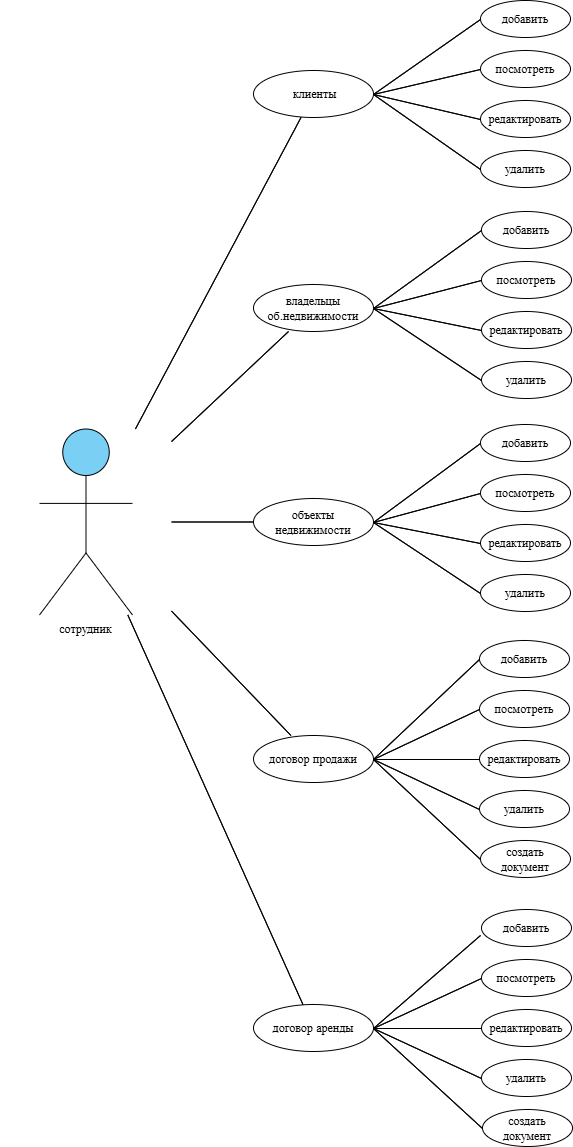
\includegraphics[width=0.73\linewidth]{диаграм_сотрудник}
	\caption{Прецеденты для сотрудника}
	\label{user_precedent_diagram:image}
\end{figure}

Руководству должны быть доступны следующие функции:
\begin{itemize}
\item	добавление сотрудников;

\item	удаление сотрудников;

\item	добавление покупателей;

\item	добавление владельцев недвижимости;

\item	добавление объектов недвижимости;

\item	просмотр информации о сотрудниках;

\item	просмотр информации о покупателях;

\item	просмотр информации о владельцах объектов недвижимости;

\item	просмотр информации о объектах недвижимости;

\item	удаление  различной информации;

\item	создание договоров аренды;

\item	создание договоров купли-продажи;

\item	удаление договоров.
\end{itemize}
\paragraph{Сценарий прецедента сотрудника «добавление информации о покупателе/арендаторе»}

Основной успешный сценарий для прецедента «добавление информации о покупателе/арендаторе».
\begin{enumerate}
\item	Открыть окно «добавить покупателя/арендатора».

\item	Заполнить данные покупателя/арендатора.

\item	Нажать кнопку «добавить»
\end{enumerate}
\paragraph{Сценарий прецедента сотрудника «просмотр информации о покупателе/арендаторе»}

Основной успешный сценарий для прецедента «просмотр информации о покупателе/арендаторе».
\begin{enumerate}
\item	Открыть окно «посмотреть покупателей/арендаторов».
\end{enumerate}
\paragraph{Сценарий прецедента сотрудника «добавление информации о продавце/арендодателе»}

Основной успешный сценарий для прецедента «добавление информации о продавце/арендодателе».
\begin{enumerate}
\item	Открыть окно «добавить продавца/арендодателя».

\item	Заполнить данные продавца/арендодателя.

\item	Нажать кнопку «добавить».
\end{enumerate}
\paragraph{Сценарий прецедента сотрудника «просмотр информации о продавце/арендодателе»}

Основной успешный сценарий для прецедента «просмотр информации о продавце/арендодателе».
\begin{enumerate}
\item Открыть окно «посмотреть продавца/арендодателя».
\end{enumerate}
\paragraph{Сценарий прецедента сотрудника «добавление объекта недвижимости»}

Основной успешный сценарий для прецедента «добавление объекта недвижимости».
\begin{enumerate}
\item	Открыть окно «добавить объект недвижимости».

\item	Заполнить информацию об объекте недвижимости.

\item	Нажать кнопку «добавить»
\end{enumerate}
\paragraph{Сценарий прецедента сотрудника «просмотр объектов недвижимости»}

Основной успешный сценарий для прецедента «просмотр объектов недвижимости».
\begin{enumerate}
\item	Открыть окно «просмотреть объекты недвижимости».
\end{enumerate}
\paragraph{Сценарий прецедента сотрудника «добавить договор купли/продажи»}

Основной успешный сценарий для прецедента «добавить договор купли/продажи».
\begin{enumerate}
\item	Открыть окно «добавить договор купли/продажи».

\item	Заполнить все данные.

\item	Нажать кнопку «добавить».
\end{enumerate}
\paragraph{Сценарий прецедента сотрудника «посмотреть договора купли/продажи»}

Основной успешный сценарий для прецедента «посмотреть договор купли/продажи».
\begin{enumerate}
\item	Открыть окно «посмотреть договор купли/продажи».

\item	Выбрать договор.

\item	Нажать кнопку «создать договор».

\item	Сохранить договор на устройстве.
\end{enumerate}
\paragraph{Сценарий прецедента сотрудника «добавить договор аренды»}

Основной успешный сценарий для прецедента «добавить договор аренды».
\begin{enumerate}
\item	Открыть окно «добавить договор аренды».

\item	Заполнить все данные.

\item	Нажать кнопку «добавить».
\end{enumerate}
\paragraph{Сценарий прецедента сотрудника «посмотреть договор аренды»}

Основной успешный сценарий для прецедента «просмотреть договора аренды».
\begin{enumerate}
\item	Открыть окно «посмотреть договор аренды».

\item	Выбрать договор.

\item	Нажать кнопку «создать договор».

\item	Сохранить договор на устройстве.
\end{enumerate}
\paragraph{Сценарий прецедента руководителя «Добавление сотрудника»}

Основной успешный сценарий для прецедента «Добавление сотрудника».
\begin{enumerate}
\item	Открыть окно «добавить сотрудника».

\item	Заполнить данные сотрудника.

\item	Нажать кнопку «добавить».
\end{enumerate}
\paragraph{Сценарий прецедента руководителя «Просмотр сотрудников»}

Основной успешный сценарий для прецедента «Просмотр сотрудников».
\begin{enumerate}
\item	Открыть окно «просмотреть сотрудников агентства».
\end{enumerate}

\subsubsection{Требования пользователя к интерфейсу приложения}

Приложение должно иметь следующие окна:
\begin{itemize}
\item	Главное окно;

\item	Окно с добавлением покупателя/арендатора;

\item	Окно с просмотром покупателей/арендаторов;

\item	Окно с добавлением продавцов/арендодателей;

\item	Окно с просмотром продавцов/арендодателей;

\item	Окно с добавлением объектов недвижимости;

\item	Окно с просмотром объектов недвижимости;

\item	Окно с добавлением сотрудников;

\item	Окно с просмотром сотрудников;

\item	Окно с добавлением договоров продажи;

\item	Окно с просмотром договоров продажи;

\item	Окно с добавлением договоров аренды;

\item	Окно с просмотром договоров аренды.
\end{itemize}
\clearpage

На рисунке ~\ref{gl_okno:image} представлен интерфейс приложения.

\begin{figure}[H]
	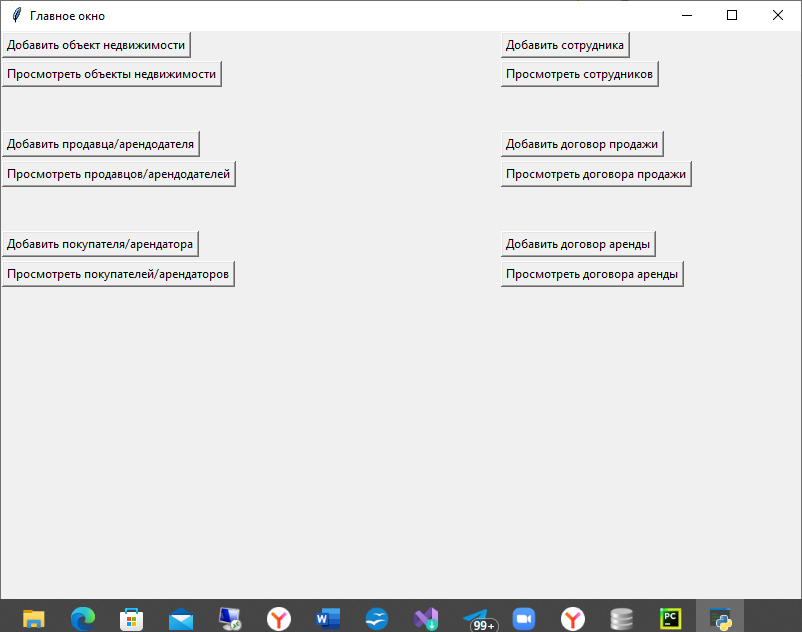
\includegraphics[width=1\linewidth]{главн_окно}
	\caption{Интерфейс приложения}
	\label{gl_okno:image}
\end{figure}


\subsubsection{Нефункциональные требования}

\paragraph{Требования к безопасности}

Необходимо устранить уязвимости, возможные для приложений:
\begin{itemize}
\item роли пользователей: Установить разные роли (администратор, агент, клиент) с соответствующими правами доступа;

\item защита от атак с перебором паролей: Внедрить блокировку учетной записи после нескольких неудачных попыток входа;

\item шифрование данных: Использовать алгоритмы шифрования для хранения конфиденциальных данных, таких как пароли и личная информация;

\item защита передачи данных: Все данные, передаваемые по сети, должны быть защищены с помощью HTTPS;

\item защита от SQL-инъекций: Использовать технологии ORM (Object-Relational Mapping) и параметризованные запросы для защиты от SQL-инъекций;

\item ведение журналов: Реализовать механизмы ведения журналов действий пользователей и администраторов для последующего анализа;

\item управление доступом к данным: Ограничить доступ пользователей к конфиденциальной информации (например, информации о других пользователях, сделках);

\item регулярные обновления: Обеспечить своевременное обновление всех библиотек и зависимостей для защиты от известных уязвимостей;

\item безопасность сервера: Хранить серверы в защищенных помещениях с ограниченным доступом;

\item резервное копирование: Регулярно делать резервные копии базы данных и важных данных;

\item обучение сотрудников: Проводить тренинги по вопросам безопасности для пользователей и сотрудников агентства;

\item соблюдение законодательства: Соблюдать местное и международное законодательство по защите персональных данных (такие как GDPR).
\end{itemize}
\paragraph{Требования к программному обеспечению}

Для создания программного решения потребуется подготовить ряд ключевых элементов: 
\begin{itemize}
\item фреймворк Laravel, обеспечивающий структуру и упрощающий разработку; 

\item среду исполнения Python, необходимую для запуска кода;

\item систему управления базами данных.
\end{itemize}
Laravel демонстрирует широкую совместимость, работая на актуальных операционных системах, таких как Windows, macOS и Linux.

\paragraph{Требования к аппаратному обеспечению}

Для работы приложения требуется дисковое пространство не менее 1 Гб. Рекомендуется использовать процессор c 2 или более ядрами и частотой 2 ГГц или выше.

\subsection{Требования к оформлению документации}

Стадии разработки программного обеспечения и требования к программной документации для вычислительной техники, комплексов и систем любого назначения и области применения регламентируются ГОСТ 19.102–77. В состав программной документации входят:
\begin{itemize}
\item	анализ предметной области;

\item	техническое задание;

\item	технический проект;

\item	рабочий проект.
\end{itemize}
\section{Технический проект}
\subsection{Выбор технологии проектирования}
\subsubsection{Паттери MVC}

MVC (Model-View-Controller) — это широко распространённый архитектурный шаблон, используемый при разработке графических пользовательских интерфейсов (GUI) и веб-приложений. Он разделяет приложение на три взаимосвязанных компонента: модель, представление и контроллер. Такое разделение позволяет упорядочить код, упростить разработку, тестирование и поддержку, а также повысить эффективность повторного использования компонентов. Рассмотрим MVC как архитектурный шаблон для разработки, выделив его сильные и слабые стороны, а также области применения.

\subsection{Выбор средств разработки}
\subsubsection{Python}

Python – это высокоуровневый, интерпретируемый, объектно-ориентированный язык программирования, который выделяется своей читаемостью и простотой. Его универсальность и богатая экосистема делают его отличным выбором для широкого спектра задач разработки. Рассмотрим Python с точки зрения выбора средств разработки, выделив его сильные и слабые стороны, а также области применения.

Преимущества Python для разработки:
\begin{itemize}
\item	читаемость и простота синтаксиса: Python разработан с акцентом на читаемость кода. Его синтаксис интуитивно понятен, что упрощает обучение и понимание кода, особенно для начинающих разработчиков. Меньше времени тратится на разбор сложных конструкций, позволяя сосредоточиться на логике программы. Это снижает порог вхождения и ускоряет процесс разработки;

\item	большая и активная экосистема библиотек и фреймворков: Python обладает огромным количеством библиотек и фреймворков для решения практически любой задачи. Это позволяет разработчикам использовать готовые решения вместо написания кода с нуля, что значительно экономит время и ресурсы. Примеры:

\item	NumPy, SciPy, Pandas: для научных вычислений и анализа данных;

\item	Django, Flask: для веб-разработки;

\item	TensorFlow, PyTorch: для машинного обучения и искусственного интеллекта;

\item	Requests: для работы с HTTP-запросами;

\item	Beautiful Soup, Scrapy: для парсинга веб-страниц;

\item	кроссплатформенность: Python работает на различных операционных системах (Windows, macOS, Linux и др.), что обеспечивает гибкость при разработке и развертывании приложений. Код, написанный на Python, может быть легко перенесен на другую платформу без значительных изменений;

\item	поддержка различных парадигм программирования: Python поддерживает объектно-ориентированное, императивное и функциональное программирование, что позволяет разработчикам выбирать наиболее подходящий стиль для решения конкретной задачи;

\item	интерпретируемость: Python – интерпретируемый язык, что означает, что код выполняется построчно без предварительной компиляции. Это упрощает отладку и позволяет быстро вносить изменения в код;

\item	большое сообщество и широкая поддержка: Python имеет огромное и активное сообщество разработчиков, которые предоставляют помощь, создают библиотеки и фреймворки, а также активно участвуют в развитии языка. Это обеспечивает широкую поддержку и доступность ресурсов для решения возникающих проблем;

\item	быстрая разработка (Rapid Prototyping): благодаря простоте синтаксиса и доступности библиотек Python идеально подходит для быстрой разработки прототипов и MVP (минимально жизнеспособного продукта).
\end{itemize}
Недостатки Python для разработки:
\begin{itemize}
\item	производительность: Python, как интерпретируемый язык, часто уступает в производительности компилируемым языкам, таким как C++ или Java. Это может быть критично для задач, требующих высокой вычислительной мощности или низкой задержки. Однако для многих задач разница в производительности не является решающим фактором, и преимущества Python в скорости разработки перевешивают этот недостаток. Кроме того, можно использовать библиотеки, написанные на C/C++, для оптимизации критических участков кода;

\item	глобальная блокировка интерпретатора (GIL): GIL ограничивает возможность параллельного выполнения кода Python в многопоточных приложениях, что может снижать производительность на многоядерных процессорах. Однако для задач, связанных с вводом-выводом (I/O), GIL не является существенным ограничением, и для достижения параллелизма можно использовать многопроцессорность или асинхронное программирование;

\item	веб-разработка: создание веб-приложений и API с использованием фреймворков, таких как Django и Flask;

\item	анализ данных и машинное обучение: обработка и анализ больших объемов данных, построение моделей машинного обучения с использованием библиотек, таких как NumPy, SciPy, Pandas, Scikit-learn, TensorFlow и PyTorch;

\item	автоматизация и скрипты: написание скриптов для автоматизации рутинных задач, администрирования систем и сетей;

\item	тестирование: автоматизация тестирования программного обеспечения с использованием фреймворков, таких как pytest и unittest;

\item	разработка игр: создание игр с использованием библиотек, таких как Pygame;

\item	научные вычисления: моделирование физических процессов, обработка изображений и сигналов с использованием библиотек, таких как NumPy, SciPy и Matplotlib;

\item	DevOps: Автоматизация процессов развертывания, мониторинга и управления инфраструктурой.

Python в сравнении с другими языками:

\item	Python против Java: Python обычно проще в изучении и использовании, чем Java, но Java может быть более производительной для некоторых задач. Java также имеет более развитую систему статической типизации, которая помогает обнаруживать ошибки на этапе компиляции;

\item	Python против C++: C++ обеспечивает более высокую производительность, чем Python, но разработка на C++ требует больше времени и усилий. Python часто используется для создания прототипов и быстрого решения задач, а C++ — для задач, требующих максимальной производительности;

\item	Python против JavaScript: JavaScript является основным языком для разработки веб-интерфейсов, а Python чаще используется для серверной части веб-приложений. Однако с появлением Node.js JavaScript также можно использовать для разработки серверной части.
\end{itemize}
Python — это мощный и универсальный язык программирования, который отлично подходит для широкого спектра задач разработки. Его читаемость, простота и богатая экосистема позволяют учитывать специфику проекта и требования к производительности, но в большинстве случаев Python будет отличным выбором.

\subsubsection{pgAdmin4}

pgAdmin 4 — это современный и многофункциональный инструмент администрирования и разработки для СУБД PostgreSQL. Это один из самых популярных и широко используемых графических пользовательских интерфейсов (GUI) для работы с PostgreSQL, предоставляющий удобный и интуитивно понятный интерфейс для выполнения различных задач, от администрирования и мониторинга до разработки и отладки. Рассмотрим pgAdmin 4 с точки зрения выбора средств разработки, подчеркнув его сильные и слабые стороны, а также целевую аудиторию.

Преимущества pgAdmin 4 для разработки:
\begin{itemize}
\item	кроссплатформенность: pgAdmin 4 можно запускать как веб-приложение в браузере, что обеспечивает кроссплатформенность и позволяет использовать его в различных операционных системах (Windows, macOS, Linux и др.) без необходимости установки дополнительных компонентов;

\item	удобный и интуитивно понятный интерфейс: интерфейс pgAdmin 4 разработан с учетом удобства пользователя. Он предоставляет визуальные инструменты для управления серверами, базами данных, таблицами, представлениями, функциями и другими объектами PostgreSQL. Навигация по интерфейсу интуитивно понятна, что облегчает выполнение различных задач;

\item	мощный редактор SQL: pgAdmin 4 оснащен мощным редактором SQL с подсветкой синтаксиса, автодополнением кода и возможностью выполнения нескольких запросов одновременно. Редактор также предоставляет инструменты для отладки SQL-кода и анализа планов запросов;

\item	визуальные инструменты для управления базами данных: pgAdmin 4 предоставляет визуальные инструменты для создания, изменения и удаления баз данных, таблиц, представлений, функций и других объектов PostgreSQL. Это упрощает процесс проектирования и разработки баз данных, особенно для начинающих разработчиков;

\item	поддержка расширений PostgreSQL: pgAdmin 4 поддерживает расширения PostgreSQL, что позволяет разработчикам использовать дополнительные функциональные возможности СУБД;

\item	мониторинг производительности: pgAdmin 4 предоставляет инструменты для мониторинга производительности PostgreSQL, что позволяет выявлять узкие места и оптимизировать работу базы данных;

\item	управление пользователями и ролями: pgAdmin 4 упрощает управление пользователями и ролями PostgreSQL, что позволяет контролировать доступ к данным и обеспечивать безопасность базы данных;

\item	резервное копирование и восстановление данных: pgAdmin 4 предоставляет инструменты для резервного копирования и восстановления данных PostgreSQL, что обеспечивает защиту данных от потери;

\item	бесплатность и открытый исходный код: pgAdmin 4 — это бесплатный инструмент с открытым исходным кодом, что позволяет использовать его без ограничений и модифицировать в соответствии с потребностями.
\end{itemize}
pgAdmin 4 — отличный выбор для разработки и администрирования баз данных PostgreSQL. Он предоставляет удобный и интуитивно понятный интерфейс с широким набором инструментов для выполнения различных задач. pgAdmin 4 особенно полезен для разработчиков, администраторов баз данных и аналитиков данных, работающих с PostgreSQL. Хотя существуют и другие альтернативные инструменты, pgAdmin 4 остается одним из самых популярных и востребованных клиентов для PostgreSQL благодаря своей функциональности, кроссплатформенности и бесплатному доступу. При выборе инструмента следует учитывать требования к ресурсам, уровень знаний и специфические потребности проекта.


\subsubsection{Фреймворк Laravel}

Laravel – это бесплатный, с открытым исходным кодом PHP-фреймворк, предназначенный для разработки современных веб-приложений, следующих архитектурному шаблону MVC (Model-View-Controller). Известный своей элегантностью, выразительностью и богатым набором встроенных инструментов, Laravel значительно упрощает и ускоряет процесс разработки, делая его популярным выбором среди PHP-разработчиков. Рассмотрим Laravel с точки зрения выбора средств разработки, выделив его сильные и слабые стороны, а также целевую аудиторию.

Преимущества Laravel для разработки:
\begin{itemize}
\item	элегантный синтаксис и выразительность: Laravel известен своим чистым и выразительным синтаксисом, который делает код легко читаемым и поддерживаемым. Это снижает когнитивную нагрузку на разработчиков и позволяет им быстрее понимать и изменять код;

\item	MVC-архитектура: Laravel использует архитектурный шаблон MVC, который разделяет приложение на три основных компонента: модель (данные), представление (интерфейс пользователя) и контроллер (логика приложения). Это облегчает организацию кода, повторное использование компонентов и тестирование;

\item	встроенная система маршрутизации: Laravel предоставляет мощную и гибкую систему маршрутизации, которая позволяет легко определять правила обработки HTTP-запросов и связывать их с соответствующими контроллерами;

\item	шаблонизатор Blade: Blade – это простой, но мощный шаблонизатор в Laravel, который позволяет создавать динамические веб-страницы с использованием PHP-кода и специальных директив. Blade обеспечивает наследование шаблонов, компоненты и другие полезные функции;

\item	миграции баз данных: Laravel предоставляет систему миграций баз данных, которая позволяет легко создавать и изменять структуру базы данных, а также отслеживать изменения в ее истории. Миграции упрощают развертывание приложения на различных средах;

\item	Artisan Console: Artisan – это консольная утилита Laravel, которая предоставляет множество полезных команд для автоматизации рутинных задач, таких как создание контроллеров, моделей, миграций, генерация кода и многое другое.

\item	тестирование: Laravel разработан с учетом тестирования и предоставляет встроенные инструменты для написания модульных и интеграционных тестов;

\item	безопасность: Laravel предоставляет встроенные инструменты для защиты от распространенных веб-угроз, таких как CSRF (Cross-Site Request Forgery), XSS (Cross-Site Scripting) и SQL-инъекции;

\item	авторизация и аутентификация: Laravel упрощает реализацию систем авторизации и аутентификации пользователей, предоставляя готовые компоненты для регистрации, входа в систему, сброса пароля и т.д.;

\item	очереди: Laravel предоставляет систему очередей для обработки задач в фоновом режиме, что позволяет разгрузить основной поток приложения и улучшить его отзывчивость;

\item	активное сообщество и документация: Laravel имеет большое и активное сообщество разработчиков, которые создают пакеты, делятся знаниями и оказывают помощь. Официальная документация Laravel хорошо написана и содержит множество примеров;

\item	пакеты (Composer): расширяемость за счет использования Composer и обширной экосистемы пакетов.
\end{itemize}
Недостатки Laravel для разработки:
\begin{itemize}
\item	изучение: хотя Laravel имеет элегантный синтаксис, изучение фреймворка может потребовать времени, особенно для начинающих PHP-разработчиков. Необходимо освоить концепции MVC, ORM, шаблонизатора и другие компоненты Laravel;

\item	производительность: Laravel, как и другие PHP-фреймворки, может уступать в производительности компилируемым языкам, таким как Java. Однако для большинства веб-приложений разница в производительности не является критической, и можно принять меры для оптимизации приложений на Laravel;

\item	размер: Laravel — довольно большой фреймворк, что может привести к увеличению размера приложения и времени загрузки.
\end{itemize}
Laravel — отличный выбор для PHP-разработчиков, которые хотят создавать современные, элегантные и масштабируемые веб-приложения. Его выразительный синтаксис, богатый набор встроенных инструментов и активное сообщество делают его одним из самых популярных PHP-фреймворков в мире. При выборе Laravel стоит учитывать требования к производительности, сложность проекта и опыт команды разработчиков. Для проектов, требующих высокой производительности или глубокой интеграции с существующей инфраструктурой, могут подойти другие фреймворки. Но в целом Laravel обеспечивает отличный баланс между функциональностью, простотой использования и производительностью.


\subsection{Архитектура программной системы}

Система состоит из следующих основных компонентов:

\subsubsection{Клиент-Приложение}

Описание: Этот компонент объединяет уровень представления (пользовательский интерфейс) и уровень приложений (бизнес-логику). Он отвечает за взаимодействие с пользователем, обработку запросов и передачу данных в базу данных.

ТЕХНОЛОГИИ:

Python: Основной язык программирования для реализации приложения.

psycopg2: Библиотека Python для подключения и взаимодействия с сервером PostgreSQL.

Tkinter: для создания простого графического интерфейса (GUI) или текстового интерфейса. 

ИЕТЕРФЕЙС ПОЛЬЗОВАТЕЛЯ:

Отображение данных о недвижимости, клиентах и сделках в виде таблицы или списка.

Предоставление форм для добавления, редактирования и удаления данных.

Реализация функциональности поиска и фильтрации данных по различным критериям.

Навигация по данным.

БИЗНЕС ЛОГИКА:

Получение данных от пользователя.

Проверка введенных данных (например, проверка формата даты, типа данных и т. д.).

Формирование SQL-запросов для взаимодействия с базой данных.

Обработка результатов запросов, полученных от базы данных.

Вывод результатов на экран.

\subsubsection{Уровень данных}

Описание: Отвечает за хранение и управление данными системы.

Технологии:

PostgreSQL: выбрана в качестве СУБД. PostgreSQL — мощная объектно-реляционная СУБД с открытым исходным кодом, отличающаяся высокой надежностью, производительностью и поддержкой стандартов SQL.

ФУНКЦИОНАЛЬНОСТЬ:

Хранение данных о недвижимости, клиентах и сделках в структурированном виде.

Обеспечение целостности данных с использованием ограничений, ключей и транзакций.

Предоставление доступа к данным через язык SQL.

Индексирование данных для ускорения поиска.

\subsubsection{Технологии и инструменты разработки}

Язык программирования: Python
СУБД: PostgreSQL

Python-библиотека для PostgreSQL: psycopg2

GUI-библиотека (опционально): Tkinter

Инструменты разработки: IDE (PyCharm), система контроля версий (Git, GitHub)

\subsubsection{Функциональность}

Операции CRUD: реализация функций для создания, чтения, обновления и удаления данных в таблицах realty, client и owner.

Поиск и фильтрация: реализация возможности поиска объектов недвижимости по различным критериям (например, по типу, адресу, цене).

Вывод данных: отображение данных в удобном формате (таблица, список).

Добавление сделок: реализация возможности добавления информации о сделках в таблицу.

\subsubsection{Перспективы развития}

Реализация более продвинутых функций поиска и фильтрации данных.

Интеграция с внешними сервисами (например, картографическими сервисами).

\subsection{Структура базы данных}

На основе анализа неформального описания предметной области были определены наборы объектов и связей. 

ОПРЕДЕЛЕНИЯ ОБЪЕКТОВ

Потенциальные объекты и атрибуты:

Каждый объект недвижимости характеризуется следующими параметрами:
\begin{itemize}
\item	код объекта недвижимости;

\item	тип сделки;

\item	регион;

\item	город;

\item	улица;

\item	номер дома;

\item	номер квартиры (если есть);

\item	площадь, кв.м;

\item	кол-во комнат;

\item	срок сдачи (если сдается);

\item	цена.
\end{itemize}
Информация о владельце объекта недвижимости включает следующее:
\begin{itemize}
\item	ФИО;

\item	паспортные данные;

\item	контактные данные;

\item	ID недвижимости.
\end{itemize}
Информация о покупателе/арендаторе включает следующее:
\begin{itemize}
\item	ФИО;

\item	паспортные данные;

\item	контактные данные.
\end{itemize}
Информация о сотруднике агентства включает следующее:
\begin{itemize}
\item	ФИО;

\item	паспортные данные;

\item	контактные данные.

\end{itemize}
Каждая сделка по покупке/аренде характеризуется следующими параметрами:
\begin{itemize}
\item	номер сделки сделки;

\item	код объекта недвижимости;

\item	данные владельца;

\item	данные покупателя/арендатора;

\item	данные сотрудника агентства;

\item	тип сделки;

\item	срок аренды (если есть);

\item	цена;

\item	дата сделки.
\end{itemize}
Сущности и отношения между ними отображены на ER-диаграмме.
\begin{figure}[H]
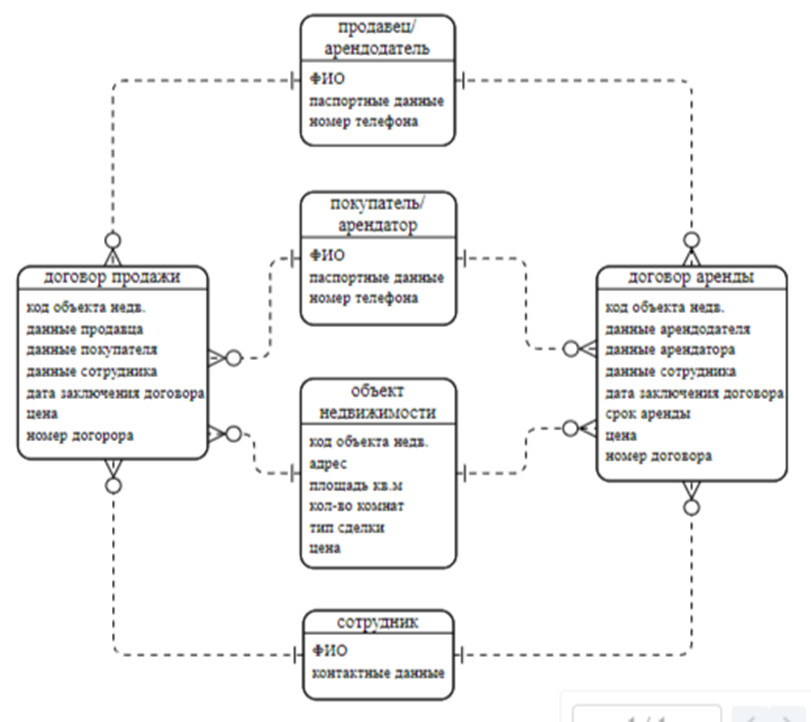
\includegraphics[width=1\linewidth]{er_diagr}
\caption{ER-диаграмма}
\label{ER_diagramma:image}
\end{figure}

\subsection{Логическое проектирование базы данных}

\subsubsection{Нормализация ER-модели данных}

Первая нормальная форма: каждый атрибут данной модели имеет только
одно значение.

Вторая форма: каждый атрибут зависит только от полного UID объекта.

Третья форма: каждый атрибут зависит только от UID своего объекта.

Объект «Продавец/арендодатель» соответствует 1NF, так как каждый атрибут имеет только одно значение.

Объект «Продавец/арендодатель» соответствует 2NF, так как каждый атрибут зависит от полного UID данного объекта.

Объект «Продавец/арендодатель» соответствует 3NF, так как каждый атрибут зависит только от UID данного объекта.

Объект «Покупатель/арендатор» соответствует 1NF, так как каждый атрибут имеет только одно значение.

Объект «Покупатель/арендатор» соответствует 2NF, так как каждый атрибут зависит от полного UID данного объекта.

Объект «Покупатель/арендатор» соответствует 3NF, так как каждый атрибут зависит только от UID данного объекта.

Объект «Объект недвижимости» соответствует 1NF, так как каждый атрибут имеет только одно значение.

Объект «Объект недвижимости» соответствует 2NF, так как каждый атрибут зависит от полного UID данного объекта.

Объект «Объект недвижимости» соответствует 3NF, так как каждый атрибут зависит только от UID данного объекта.

Объект «Сотрудник» соответствует 1NF, так как каждый атрибут имеет только одно значение.

Объект «Сотрудник» соответствует 2NF, так как каждый атрибут зависит от полного UID данного объекта.

Объект «Сотрудник» соответствует 3NF, так как каждый атрибут зависит только от UID данного объекта.

Объект «Договор продажи» соответствует 1NF, так как каждый атрибут имеет только одно значение.

Объект «Договор продажи» соответствует 2NF, так как каждый атрибут зависит от полного UID данного объекта.

Объект «Договор продажи» соответствует 3NF, так как каждый атрибут зависит только от UID данного объекта.

Объект «Договор аренды» соответствует 1NF, так как каждый атрибут имеет только одно значение.


На основе ER-модели данных в онлайн-сервисе Lucidcharts построена реляционная модель данных, показанная на рисунке \ref{exchange_scheme:image}.

\begin{figure}[H]
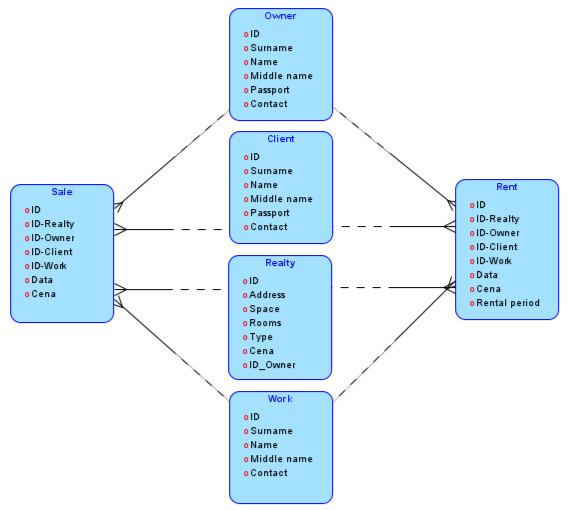
\includegraphics[width=0.8\linewidth]{model_dan}
\caption{Реляционная модель данных}
\label{exchange_scheme:image}
\end{figure}

Названия таблиц и названия столбцов каждой таблицы приведены в таблицах 3.1 -3.6.

\begin{xltabular}{\textwidth}{|l|l|X|X|}
	\caption{Владелец объекта недвижимости\label{owner:table}}\\ \hline
	\centrow Кеу Type & \centrow Optionality & \centrow Column name & \centrow Data type \\ \hline
	\thead{1} & \thead{2} & \centrow 3 & \centrow 4 \\ \hline
	\endfirsthead
	\thead{1} & \thead{2} & \centrow 3 & \centrow 4 \\ \hline
	\finishhead
	\ pk & * & Surname & TEXT \\ \hline
	& * & Name & TEXT \\ \hline
	& * & Middle name & TEXT \\ \hline
	& * & Passport & INTEGER \\ \hline
	& * & Contact & INTEGER \\ \hline
\end{xltabular}



\begin{xltabular}{\textwidth}{|l|l|X|X|}
	\caption{Клиент\label{client:table}}\\ \hline
	\centrow Кеу Type & \centrow Optionality & \centrow Column name & \centrow Data type \\ \hline
	\thead{1} & \thead{2} & \centrow 3 & \centrow 4 \\ \hline
	\endfirsthead
	\thead{1} & \thead{2} & \centrow 3 & \centrow 4 \\ \hline
	\finishhead
	\ pk & * & Surname & TEXT \\ \hline
	& * & Name & TEXT \\ \hline
	& * & Middle name & TEXT \\ \hline
	& * & Passport & INTEGER \\ \hline
	& * & Contact & INTEGER \\ \hline
\end{xltabular}



\begin{xltabular}{\textwidth}{|l|l|X|X|}
	\caption{Объект недвижимости\label{realty:table}}\\ \hline
	\centrow Кеу Type & \centrow Optionality & \centrow Column name & \centrow Data type \\ \hline
	\thead{1} & \thead{2} & \centrow 3 & \centrow 4 \\ \hline
	\endfirsthead
	\thead{1} & \thead{2} & \centrow 3 & \centrow 4 \\ \hline
	\finishhead
	\ pk & * & Address & TEXT \\ \hline
	& * & Space & TEXT \\ \hline
	& * & Rooms & INTEGER \\ \hline
	& * & Type & TEXT \\ \hline
	& * & Cena & INTEGER \\ \hline
	& * & ID owner & INTEGER \\ \hline
\end{xltabular}

\begin{xltabular}{\textwidth}{|l|l|X|X|}
	\caption{Сотрудник агентства\label{wort:table}}\\ \hline
	\centrow Кеу Type & \centrow Optionality & \centrow Column name & \centrow Data type \\ \hline
	\thead{1} & \thead{2} & \centrow 3 & \centrow 4 \\ \hline
	\endfirsthead
	\thead{1} & \thead{2} & \centrow 3 & \centrow 4 \\ \hline
	\finishhead
	\ pk & * & Surname & TEXT \\ \hline
	& * & Name & TEXT \\ \hline
	& * & Middle name & TEXT \\ \hline
	& * & Contact & INTEGER \\ \hline
\end{xltabular}

\begin{xltabular}{\textwidth}{|l|l|X|X|}
	\caption{Договор продажи\label{sale:table}}\\ \hline
	\centrow Кеу Type & \centrow Optionality & \centrow Column name & \centrow Data type \\ \hline
	\thead{1} & \thead{2} & \centrow 3 & \centrow 4 \\ \hline
	\endfirsthead
	\thead{1} & \thead{2} & \centrow 3 & \centrow 4 \\ \hline
	\finishhead
	\ pk & * & Realty & TEXT \\ \hline
	& * & Owner & TEXT \\ \hline
	& * & Client & TEXT \\ \hline
	& * & Work & TEXT \\ \hline
	& * & Data & DATE \\ \hline
	& * & Cena & INTEGER \\ \hline
\end{xltabular}

\begin{xltabular}{\textwidth}{|l|l|X|X|}
	\caption{Договор аренды\label{renta:table}}\\ \hline
	\centrow Кеу Type & \centrow Optionality & \centrow Column name & \centrow Data type \\ \hline
	\thead{1} & \thead{2} & \centrow 3 & \centrow 4 \\ \hline
	\endfirsthead
	\thead{1} & \thead{2} & \centrow 3 & \centrow 4 \\ \hline
	\finishhead
	\ pk & * & Realty & TEXT \\ \hline
	& * & Owner & TEXT \\ \hline
	& * & Client & TEXT \\ \hline
	& * & Work & TEXT \\ \hline
	& * & Data & DATE \\ \hline
	& * & Cena & INTEGER \\ \hline
	& * & Rental period & TEXT \\ \hline
\end{xltabular}

\ifПрактика{}\else{
   \section{Рабочий проект}
\subsection{Описание классов и функций}
\begin{lstlisting}[language=Python]
def open_add_window():  Открывает новое окно (Toplevel) для добавления информации о недвижимости в базу данных.

def add_realty(): Добавляет информацию об объекте недвижимости в базу данных. Эта функция определена внутри 

open_add_window() и имеет доступ к виджетам этого окна.

def open_salee_window(): открывает новое окно (Toplevel) для просмотра данных о продажах из таблицы sale базы данных.

def create_agreement(): создает договор купли-продажи на основе выбранной записи в списке продаж.

def open_view_window(): эта функция отвечает за создание и отображение окна просмотра объектов недвижимости. Она извлекает данные об объектах из базы данных и отображает их в окне с возможностью прокрутки.

def open_work_window(): эта функция создает окно для добавления информации о новом сотруднике.

def add_employee(): эта функция отвечает за получение данных о новом сотруднике из полей ввода, проверку (хотя бы минимальную) и добавление этой информации в таблицу employee в базе данных.


def open_worker_window(): эта функция отвечает за создание и отображение окна для просмотра списка сотрудников, хранящегося в базе данных.

def open_buy_window(): эта функция отвечает за создание окна, предназначенного для добавления информации о новом покупателе (или арендаторе). Она создает элементы интерфейса, необходимые для ввода данных о покупателе.

def add_client(): эта функция предназначена для добавления информации о новом клиенте (покупателе/арендаторе) в базу данных. Она собирает данные из полей ввода, выполняет минимальную проверку и добавляет запись в таблицу client.

def open_buyer_window(): эта функция открывает окно для просмотра списка клиентов (покупателей/арендаторов), извлекая данные из базы данных и отображая их.

def open_sell_window(): эта функция отвечает за создание окна, в котором пользователь может ввести данные о новом владельце (продавце/арендодателе) недвижимости.

def open_seller_window(): эта функция создает окно для просмотра списка владельцев (продавцов/арендодателей) недвижимости, извлекая данные из базы данных и отображая их в виде списка.

def open_sale_window(): эта функция отвечает за создание окна для ввода данных о новой продаже (заключении договора купли-продажи) и добавления этой информации в базу данных.

def add_sale(): Определяет функцию, которая будет вызываться при нажатии кнопки «Добавить». Эта функция собирает данные из полей ввода, проверяет их и добавляет новую запись в таблицу sale в базе данных.

def generate_sale_agreement(row): эта функция генерирует текст договора купли-продажи на основе данных, полученных из базы данных. Она принимает строку данных (row) в качестве аргумента и формирует текстовое представление договора, готовое к отображению или печати.

def open_salee_window(): эта функция отвечает за создание окна для просмотра информации о существующих договорах купли-продажи. Она извлекает данные о продажах из базы данных, отображает их в виде списка и предоставляет возможность сгенерировать текст договора для выбранной продажи.

def save_agreement(): эта функция позволяет сохранить сгенерированный текст договора (хранящийся в переменной agreement) в текстовый файл, выбранный пользователем с помощью диалогового окна сохранения файла.

def open_rent_window(): эта функция отвечает за создание окна, предназначенного для ввода информации о договоре аренды. 

def add_renta(): эта функция предназначена для добавления данных о новом договоре аренды в базу данных. Она собирает информацию из полей ввода в графическом интерфейсе, а затем вставляет эту информацию в таблицу renta. Также добавляет сообщение об успешном выполнении и закрывает окно.

def generate_rent_agreement(row): эта функция генерирует текст договора аренды на основе данных, полученных из строки базы данных. Функция формирует текст договора, который можно отобразить пользователю или сохранить в файл.

def open_rentt_window(): эта функция создает окно для просмотра договоров аренды. Она извлекает данные из базы данных и отображает их в виджете Listbox. Также предоставляет возможность сгенерировать договор аренды на основе выбранной записи.

save_agreement(): эта функция позволяет сохранить сгенерированный текст договора аренды (который хранится в переменной agreement) в текстовом файле. Пользователь может выбрать место и имя файла с помощью стандартного диалогового окна сохранения файла.
\end{lstlisting}  

\subsection{Тестирование разработанной программной системы}

Для работы пользователей с созданной базой данных было разработано десктопное приложение для ОС Windows. Для разработки приложения использовался язык программирования Python с фреймворком Qt, в состав которого входят библиотеки для разработки графического интерфейса и средства взаимодействия с базами данных.

Структура приложения показана на рисунках 4.13 – 4.30.

На рисунке \ref{главн_окно:image} представлено главное окно программы.

\begin{figure}[H]
\center{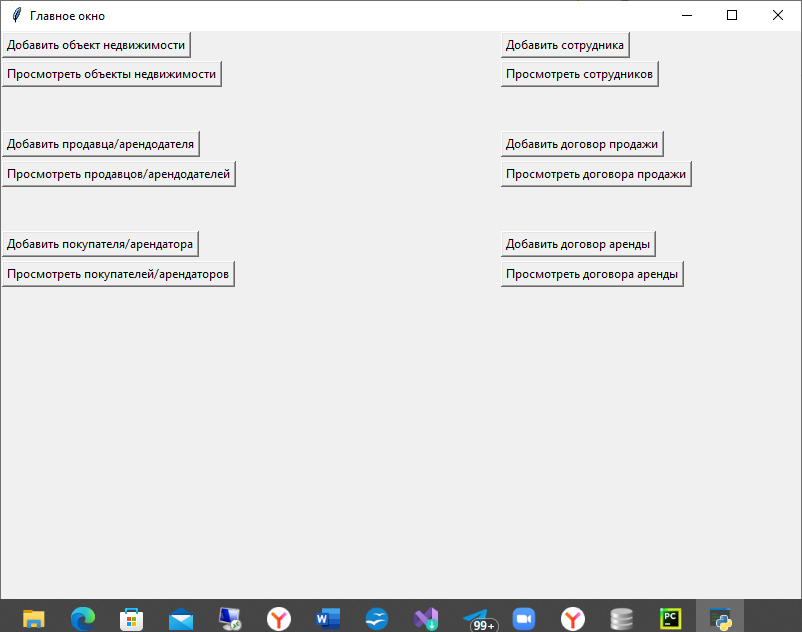
\includegraphics[width=0.8\linewidth]{главн_окно}}
\caption{Главное окно программы}
\label{главн_окно:image}
\end{figure}

На рисунке \ref{объект:image} представлено окно для добавления объектов недвижимости.

\begin{figure}[H]
	\center{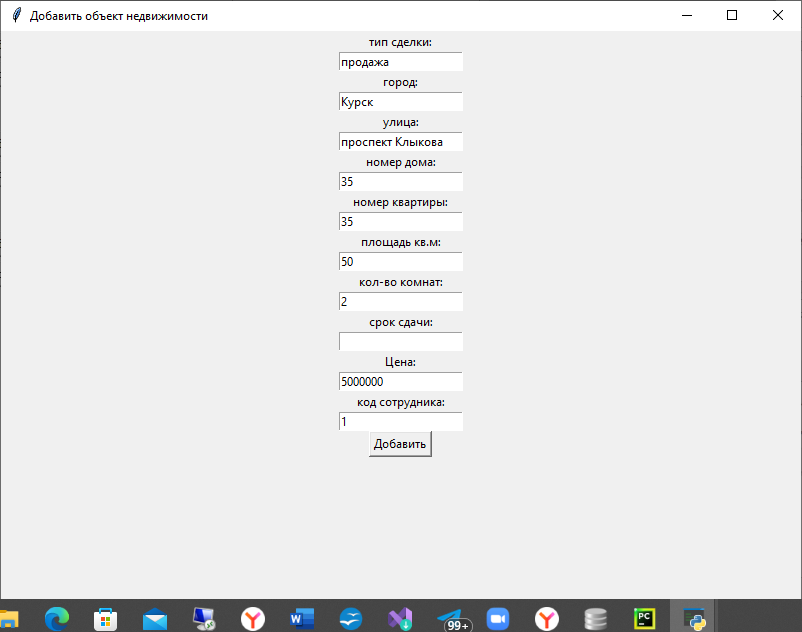
\includegraphics[width=0.8\linewidth]{объект}}
	\caption{Окно для добавления объектов недвижимости}
	\label{объект:image}
\end{figure}

На рисунке \ref{РОбъект:image} представлен результат добавления объекта недвижимости.

\begin{figure}[H]
	\center{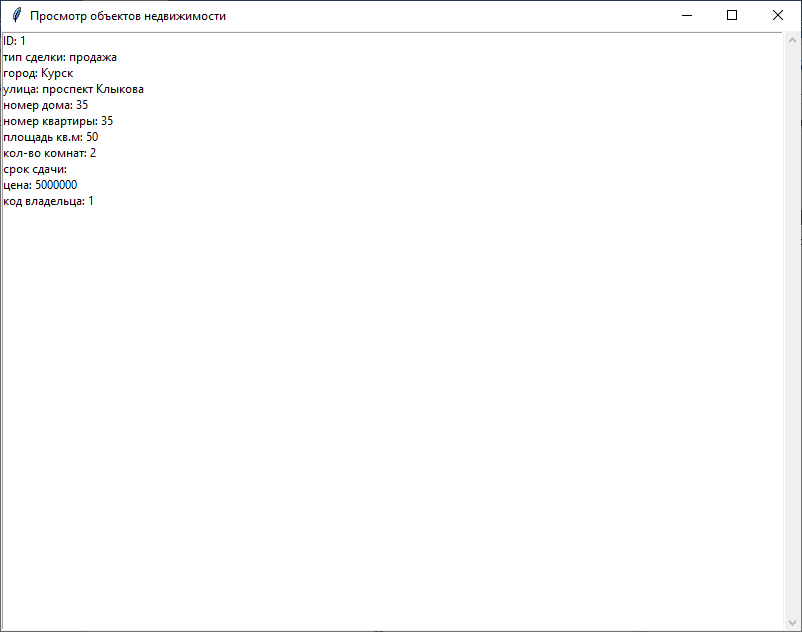
\includegraphics[width=0.8\linewidth]{РОбъект}}
	\caption{Результат добавления объекта недвижимости}
	\label{РОбъект:image}
\end{figure}

На рисунке \ref{номердома:image} представлена попытка ввести некорректные данные в поле номер дома.

\begin{figure}[H]
	\center{
\includegraphics[width=0.4\linewidth]{номердома}}
	\caption{Попытка ввести некорректные данные в поле номер дома}
	\label{номердома:image}
\end{figure}

На рисунке \ref{невсеполя:image} представлена попытка добавить данные, не заполнив все поля.

\begin{figure}[H]
	\center{
\includegraphics[width=0.4\linewidth]{невсеполя}}
	\caption{Попытка добавить данные, не заполнив все поля}
	\label{невсеполя:image}
\end{figure}\\

На рисунке \ref{продавец:image} представлено окно для добавления данных продавца/арендадателя.

\begin{figure}[H]
	\center{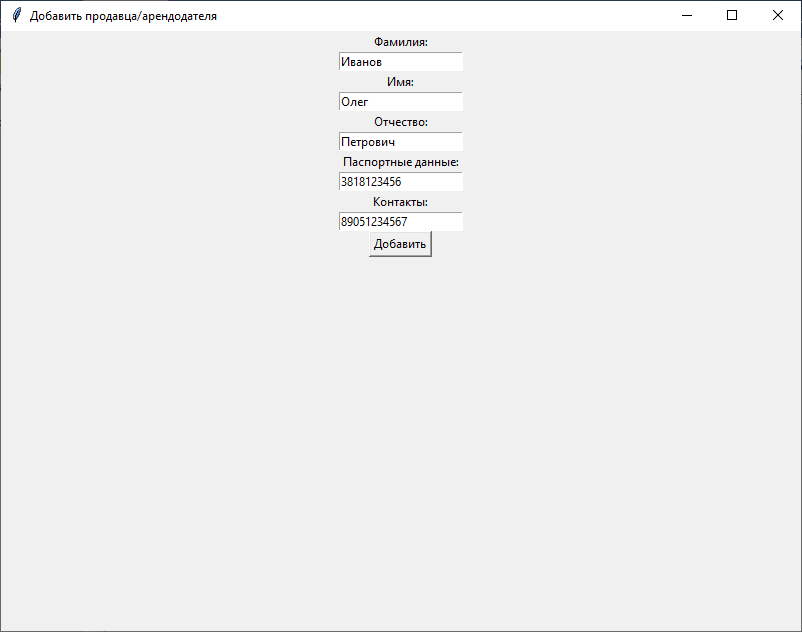
\includegraphics[width=0.8\linewidth]{продавец}}
	\caption{Окно для добавления данных продавца/арендадателя}
	\label{продавец:image}
\end{figure}

На рисунке \ref{РПродавец:image} представлен результат добавления данных продавца/арендадателя.

\begin{figure}[H]
	\center{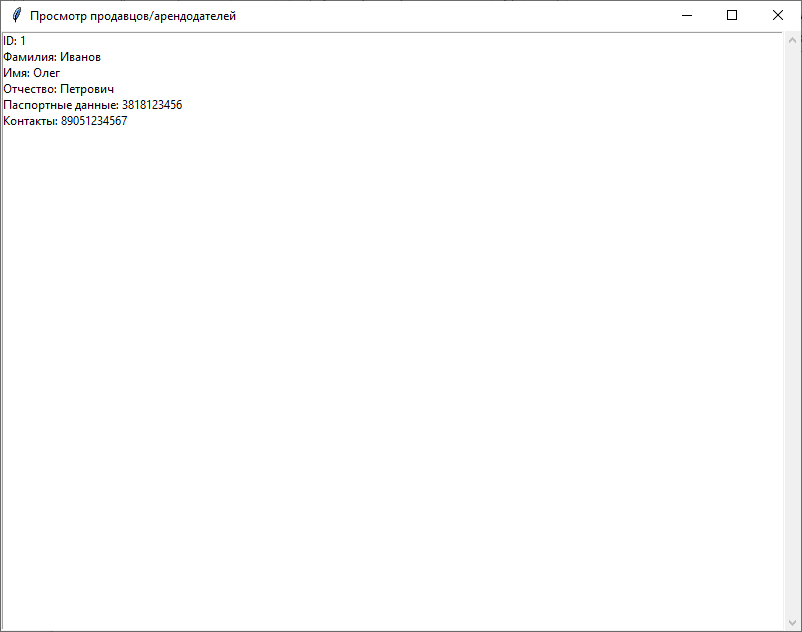
\includegraphics[width=0.8\linewidth]{РПродавец}}
	\caption{Результат добавления данных продавца/арендадателя}
	\label{РПродавец:image}
\end{figure}

На рисунке \ref{покупатель:image} представлено окно для добавления данных покупателя/арендатора.

\begin{figure}[H]
	\center{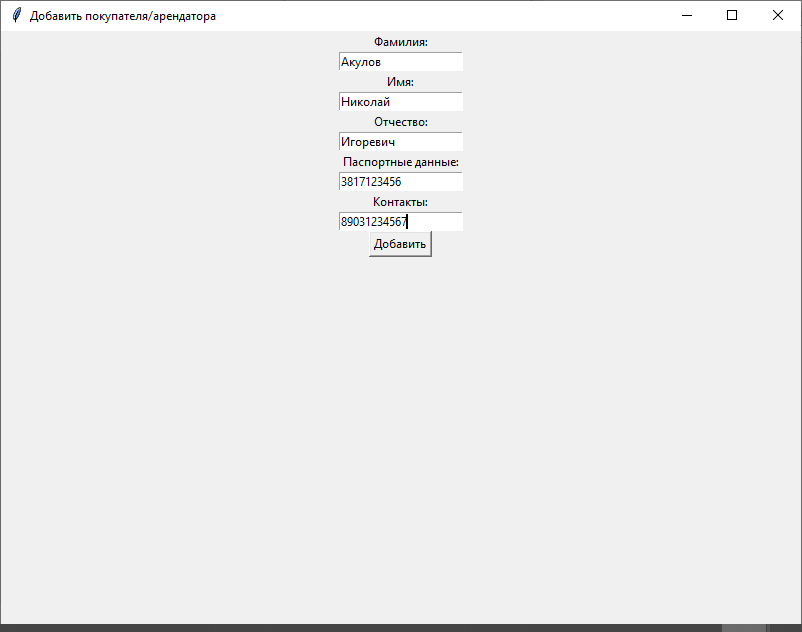
\includegraphics[width=0.8\linewidth]{Покупатель}}
	\caption{Окно для добавления данных покупателя/арендатора}
	\label{покупатель:image}
\end{figure}

На рисунке \ref{рпокпатель:image} представлен результат добавления данных покупателя/арендатора.

\begin{figure}[H]
	\center{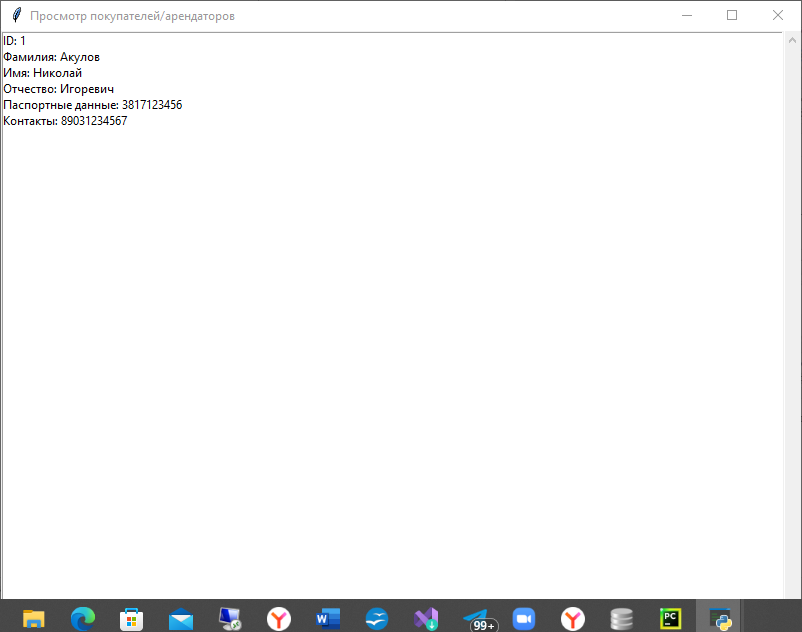
\includegraphics[width=0.8\linewidth]{РПокупатель}}
	\caption{Результат добавления данных покупателя/арендатора}
	\label{рпокупатель:image}
\end{figure}

На рисунке \ref{сотрудник:image} представлено окно для добавления данных сотрудника.

\begin{figure}[H]
	\center{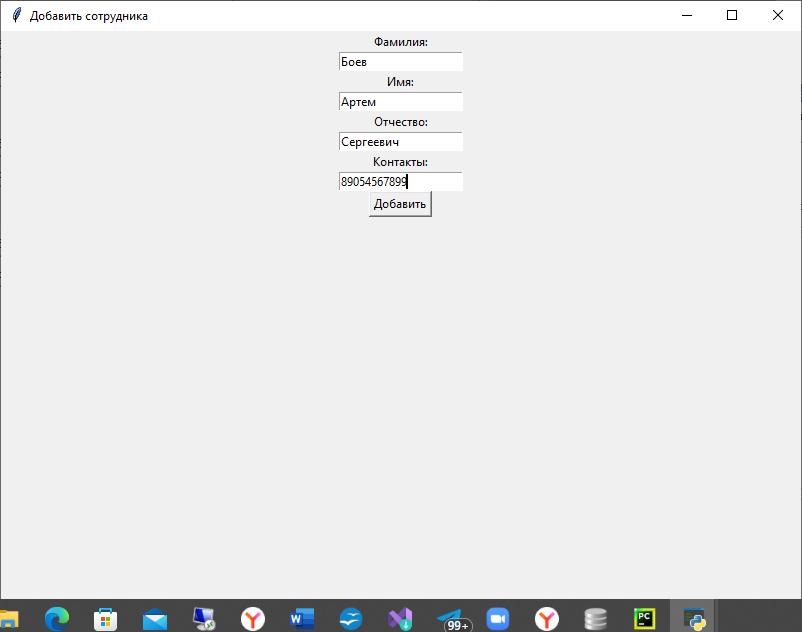
\includegraphics[width=0.8\linewidth]{Сотрудник}}
	\caption{Окно для добавления данных сотрудника}
	\label{сотрудник:image}
\end{figure}

На рисунке \ref{рсотрудник:image} представлен результат добавления данных сотрудника.

\begin{figure}[H]
	\center{
\includegraphics[width=0.8\linewidth]{РСотрудник}}
	\caption{Результат добавления данных сотрудника}
	\label{рсотрудник:image}
\end{figure}

На рисунке \ref{продажи:image} представлено окно для добавления данных договора продажи.

\begin{figure}[H]
	\center{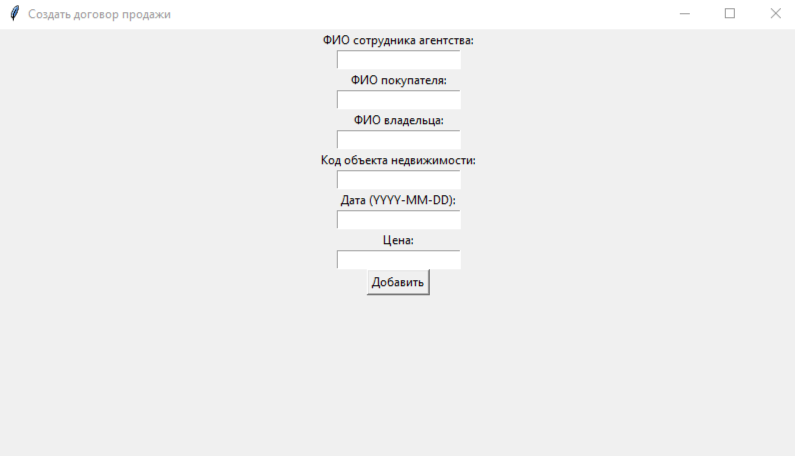
\includegraphics[width=0.8\linewidth]{Продажи}}
	\caption{Окно для добавления данных договора продажи}
	\label{продажи:image}
\end{figure}

На рисунке \ref{рпродажи:image} представлены данные для создания договора продажи.

\begin{figure}[H]
	\center{
\includegraphics[width=0.8\linewidth]{РПродажи}}
	\caption{Данные для создания договора продажи}
	\label{рпродажи:image}
\end{figure}

На рисунке \ref{договорП:image} представлен созданный договор продажи.

\begin{figure}[H]
	\center{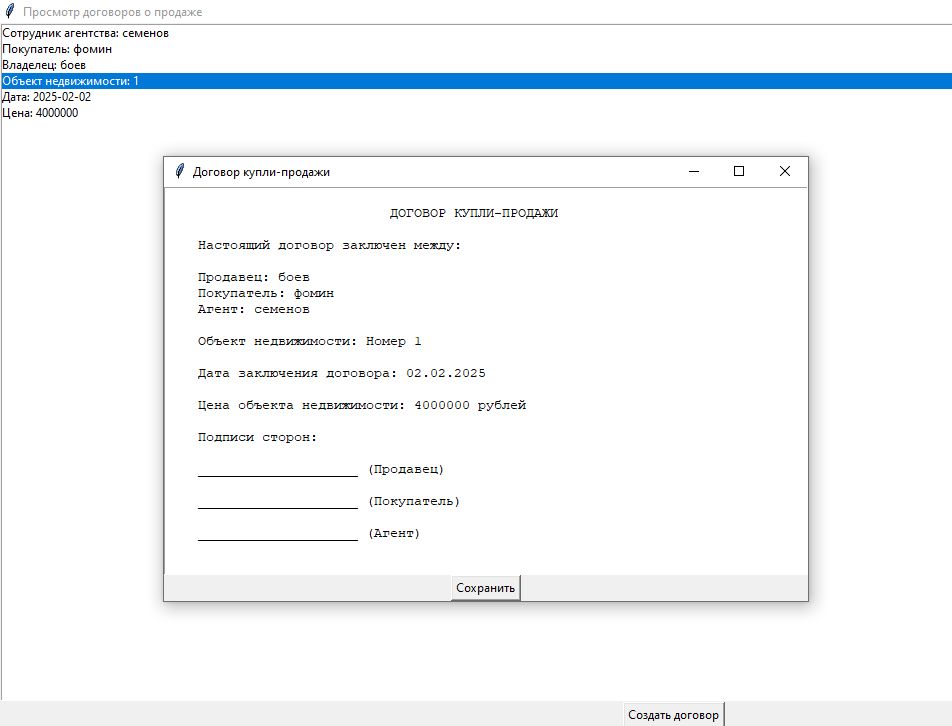
\includegraphics[width=0.8\linewidth]{ДоговорП}}
	\caption{Созданный договор продажи}
	\label{договорП:image}
\end{figure}

На рисунке \ref{аренда:image} представлено окно для добавления данных договора аренды.

\begin{figure}[H]
	\center{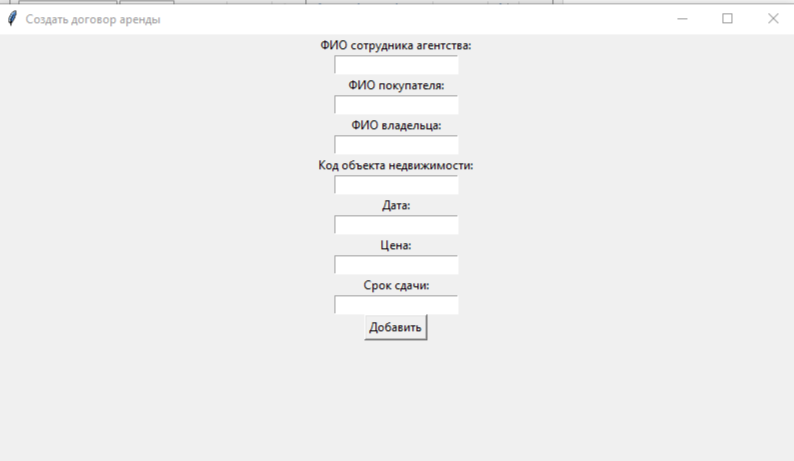
\includegraphics[width=0.8\linewidth]{Аренда}}
	\caption{Окно для добавления данных договора аренды}
	\label{аренда:image}
\end{figure}

На рисунке \ref{раренда:image} представлены данные для создания договора аренды.

\begin{figure}[H]
	\center{
\includegraphics[width=0.8\linewidth]{РАренда}}
	\caption{Данные для создания договора аренды}
	\label{раренда:image}
\end{figure}

На рисунке \ref{даренда:image} представлен созданный договор аренды.

\begin{figure}[H]
	\center{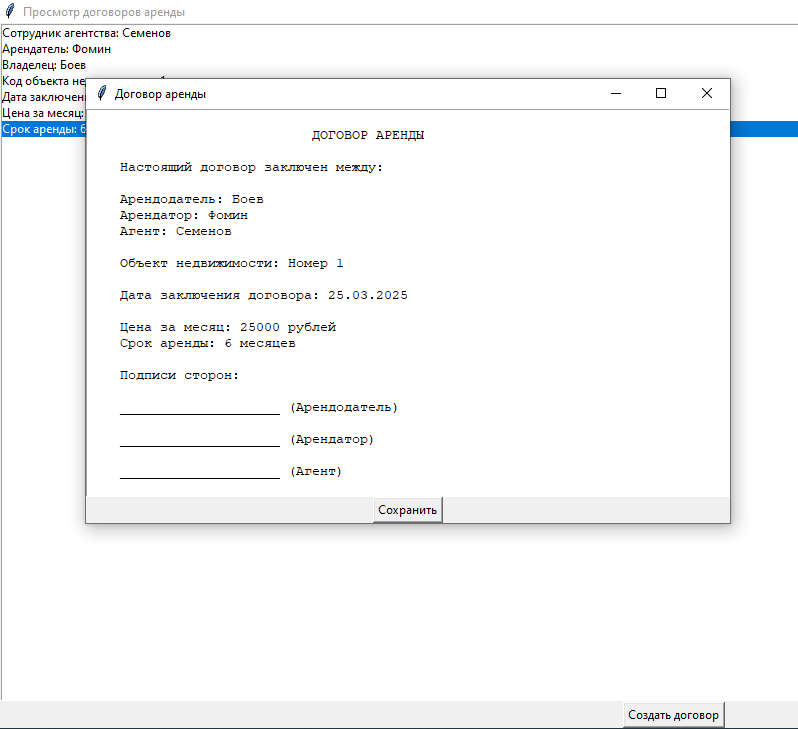
\includegraphics[width=0.8\linewidth]{ДоговорА}}
	\caption{Созданный договор аренды}
	\label{даренда:image}
\end{figure}\\

На рисунке \ref{успех:image} представлено уведомление об успешной загрузке данных в базу данных.

\begin{figure}[H]
	\center{
\includegraphics[width=0.4\linewidth]{успех}}
	\caption{Уведомление об успешной загрузке данных в базу данных}
	\label{успех:image}
\end{figure}

На рисунке \ref{пустой:image} представлена попытка создать пустой договор.

\begin{figure}[H]
	\center{
\includegraphics[width=0.4\linewidth]{пустойД}}
	\caption{Попытка создать пустой договор}
	\label{пустой:image}
\end{figure}
   \section*{ЗАКЛЮЧЕНИЕ}
\addcontentsline{toc}{section}{ЗАКЛЮЧЕНИЕ}
Целью данной работы являлось проектирование базы данных агентства недвижимости и разработка приложения для доступа к этой базе данных.

При проектировании базы данных и разработке приложения были решены следующие задачи:

-  исследование предметной области;

-  проектирование базы данных;

-  создание базы данных;

-  заполнение базы данных информацией;

-  разработка интерфейса;

-  реализация приложения.

Результатом выполнения данной работы является десктопное приложение для работы пользователей с базой данных агентства недвижимости. При проектировании базы данных использован ER-подход к проектированию реляционных баз данных. Интерфейс приложения содержит: главную форму для вывода таблицы, форму для просмотра данных и редактирования записей базы данных, форму для добавления объектов недвижимости, их владельцах, покупателях и тд.

Все требования были полностью реализованы в данном программном продукте.

Все задачи, поставленные в начале проектирования проекта, были также решены.
}\fi
\addcontentsline{toc}{section}{СПИСОК ИСПОЛЬЗОВАННЫХ ИСТОЧНИКОВ}

\begin{thebibliography}{9}

    \bibitem{python} Кузнецов С.Д. Базы данных: учебник для студ. учреждений высш. проф. образования / С.Д. Кузнецов. — 2-е изд., испр. — М.: Издательский центр «Академия», 2010. — 496 с.
    \bibitem{python} Дейт, К. Дж. Введение в системы баз данных = An Introduction to Database Systems / К. Дж. Дейт. — 8-е изд. — М.: Вильямс, 2006. — 1328 с. (Общая теория баз данных)
    \bibitem{python} Коннолли, Т., Бегг, К. Базы данных. Проектирование, реализация и сопровождение. Теория и практика. 3-е изд. / Т. Коннолли, К. Бегг. — М.: Вильямс, 2003. — 816 с. (Общая теория баз данных)
    \bibitem{python} Рамкришнан Р., Гехре Д. Управление базами данных = Database Management Systems / Р. Рамкришнан, Д. Гехре. — 3-е изд. — М.: Вильямс, 2003. — 1056 с. (Общая теория баз данных)
	\bibitem{python} Васильев А.Н. Python на примерах. Практический курс программирования. — СПб.: Наука и техника, 2017. — 432 с. (Основы языка Python)
	\bibitem{python} Бизли Д.М. Справочник по Python (4-е издание). — Addison-Wesley Professional, 2009. — 704 страницы. (Справочник по Python)
	\bibitem{python} Расперри П.Л., Расин Б. Сборник рецептов по анализу данных на Python — O’Reilly Media, 2015. — 514 страниц. (Рецепты по анализу данных на Python)
	\bibitem{python} Петров А.А. Анализ предметной области «Агентство недвижимости» и разработка концептуальной модели базы данных // Вестник [Название университета/организации]. — 2020. — № 3. — С. 45-52. (Анализ предметной области)
	\bibitem{python} Сидорова Е.В. Проектирование реляционной базы данных для управления недвижимостью // Информационные технологии. — 2019. — № 12. — С. 67-74. (Проектирование реляционных БД) 
	\bibitem{python} Иванов И.И., Козлов П.С. Методы оптимизации запросов в базах данных агентств недвижимости // Системы управления базами данных. — 2021. — № 2. — С. 102-110. (Оптимизация запросов)
	\bibitem{python} Смирнов П.А. Применение ER-диаграмм для моделирования баз данных агентств недвижимости // Современные научные исследования и инновации. – 2018. – № 5. (ER-диаграммы)
	\bibitem{python} Васильев С.В. Особенности построения баз данных для информационных систем агентств недвижимости // Наука и образование: сохраняя прошлое, создаём будущее. – 2022. – С. 88-90. (Особенности БД для агентств)
	\bibitem{python} Борисова О.И. Проблемы внедрения и использования современных баз данных в агентствах недвижимости // Экономика и управление в XXI веке. – 2019. – С. 123-126. (Проблемы внедрения)
	\bibitem{python} Официальная документация Python. — URL: https://docs.python.org/3/ (дата обращения: 15.05.2024). (Официальная документация)
	\bibitem{python} Официальная документация SQLite. — URL: https://www.sqlite.org/docs.html (дата обращения: 15.05.2024). (Если вы используете SQLite)
	\bibitem{python} psycopg.org — адаптер PostgreSQL для Python. — URL: https://www.psycopg.org/ (дата обращения: 15.05.2024). (Если вы используете PostgreSQL)
	\bibitem{python} Учебник по SQL [Электронный ресурс] // W3Schools. — URL: https://www.w3schools.com/sql/ (дата обращения: 15.05.2024). (Основы SQL)
	\bibitem{python} Настоящие уроки Python — URL: https://realpython.com/ (дата обращения: 15.05.2024) (Уроки Python)
	\bibitem{python}pandas.pydata.org — библиотека Python для анализа данных. — URL: https://pandas.pydata.org/ (дата обращения: 15.05.2024) (Если вы используете Pandas)
\end{thebibliography}

\ifВКР{\appendix{Представление графического материала}

Графический материал, выполненный на отдельных листах,
изображен на рисунках А.1--А.\arabic{числоПлакатов}.
\setcounter{числоПлакатов}{0}

\renewcommand{\thefigure}{А.\arabic{figure}} % шаблон номера для плакатов



\begin{плакат}
    
\includegraphics[width=0.82\linewidth]{плакат1}
    \заголовок{Сведения о ВКРБ}
    \label{pl1:image}      
\end{плакат}

\begin{плакат}
    
\includegraphics[width=0.82\linewidth]{плакат2}
    \заголовок{Цель и задачи разработки}
    \label{pl2:image}      
\end{плакат}

\begin{плакат}
    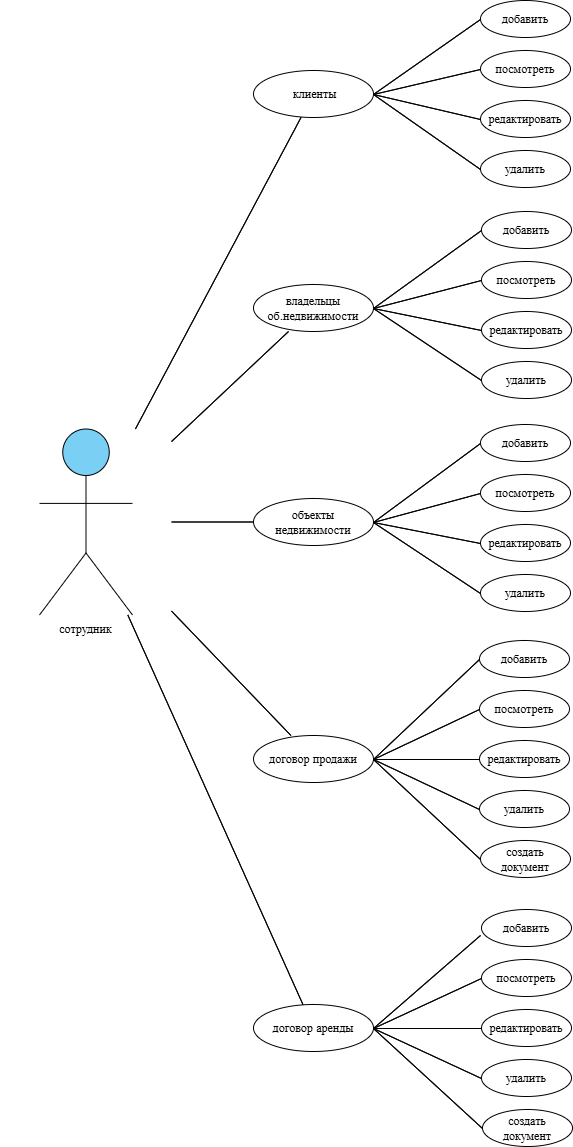
\includegraphics[width=0.73\linewidth]{диаграм_сотрудник}
    \заголовок{диаграмма прецедентов}
    \label{pl3:image}      
\end{плакат}

\begin{плакат}
    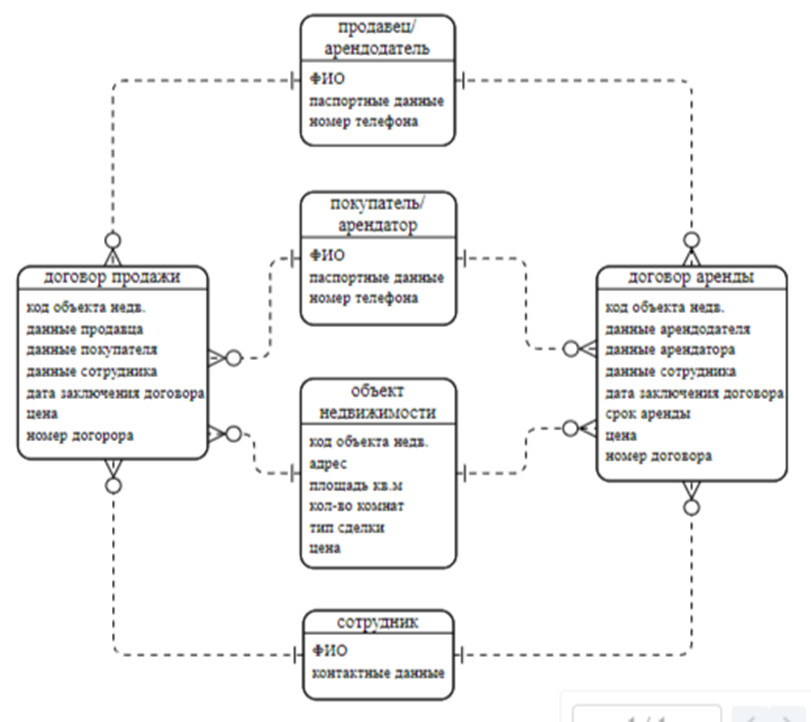
\includegraphics[width=0.82\linewidth]{er_diagr}
    \заголовок{Концептуальная модель предметной области}
    \label{pl4:image}      
\end{плакат}

\begin{плакат}
	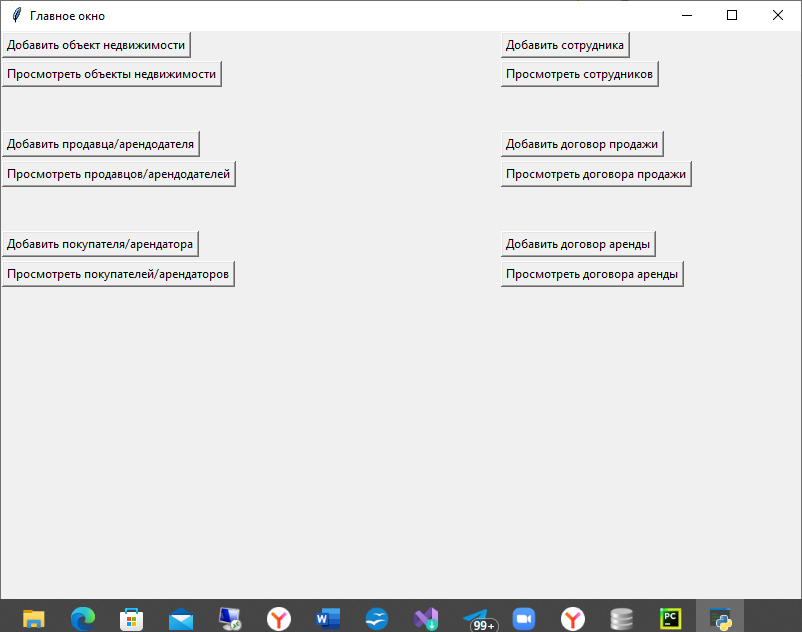
\includegraphics[width=0.82\linewidth]{главн_окно}
	\заголовок{Интерфейс приложения}
	\label{pl5:image}      
\end{плакат}

\begin{плакат}
	
\includegraphics[width=0.82\linewidth]{плакат6}
	\заголовок{Заключение}
	\label{pl6:image}      
\end{плакат}

}\fi
\ifПрактика{}\else{\appendix{Фрагменты исходного кода программы}

main.py
\lstinputlisting[language=Python, frame=none]{kod/main.py}

\ifВКР{
\newpage
\addcontentsline{toc}{section}{На отдельных листах (CD-RW в прикрепленном конверте)}
\noindent
\begin{tabular}{p{5.8cm}C{4.8cm}C{4.8cm}}
   Автор ВКР & \lhrulefill{\fill} & \fillcenter\Автор \\
            \setarstrut{\footnotesize}
           & \footnotesize{(подпись, дата)} & \\
            \restorearstrut
   Руководитель ВКР & \lhrulefill{\fill} & \fillcenter\Руководитель \\
            \setarstrut{\footnotesize}
           & \footnotesize{(подпись, дата)} & \\
            \restorearstrut
   Нормоконтроль & \lhrulefill{\fill} & \fillcenter\Нормоконтроль \\
            \setarstrut{\footnotesize}
           & \footnotesize{(подпись, дата)} & \\
            \restorearstrut
\end{tabular}
\vskip 2cm
\begin{center}
\textbf{Место для диска}
\end{center}
}\fi
}\fi
\end{document}
